\documentclass[compress,8pt]{beamer}
\usepackage[latin1]{inputenc}
\usepackage[round,authoryear]{natbib}
\bibliographystyle{apalike}

% \usepackage[scaled]{helvet} % official font size

\setbeamersize{text margin left=2em}  % <- like this
\setbeamersize{text margin right=2em} % <- like this

\usepackage{color}
\usepackage{bm}
\usepackage{multimedia}
\usepackage{latexsym} 
\usepackage{graphicx} 
\frenchspacing 
\usepackage{array}
\usepackage{amsmath}
\usepackage{amssymb}
\usepackage{amsthm}
\usepackage{mathrsfs}
\usepackage[dvips]{epsfig}
\usepackage{multirow}
\usepackage{booktabs}
\usepackage{epsf}
\usepackage{mathrsfs}
\usepackage{bm}
\usepackage{enumerate}
\usepackage{subfigure}
\usepackage{float}
\usepackage{caption}
\usepackage{picture}
\usepackage{verbatim}
\usepackage{listings}
\usepackage{indentfirst}
\usepackage{framed,color}
\usepackage{centernot}
\usepackage{graphicx}
\usepackage{animate}
\usepackage{varwidth}
\usepackage{xcolor}

\lstset{frame=single, language=python, numberstyle=\footnotesize,
basicstyle=\footnotesize, commentstyle=\footnotesize}

\newenvironment{rcases}
  {\left.\begin{aligned}}
  {\end{aligned}\right\rbrace}

\usetheme{Berlin}
\usecolortheme{dove} 

\definecolor{dark_gray}{rgb}{0.3, 0.3, 0.3} 
\definecolor{light_gray}{rgb}{0.92, 0.92, 0.92} 
% \setbeamercolor{titlelike}{parent=structure,fg=black,bg=light_gray}
% \setbeamercolor{frametitle}{bg=light_gray}
% \setbeamercolor{structure}{bg=light_gray}
\setbeamercolor{bgcolor}{fg=white,bg=dark_gray} % color footline
\setbeamercolor{bgcolor_dark}{fg=black,bg=dark_gray} % color footline

% \setbeamertemplate{headline}{\vskip40pt} % no section subsection navigation bar. Spacing after frametitle
\setbeamertemplate{headline} % no section subsection navigation bar. Spacing after frametitle
{

\vspace{0.5cm}

    \hfill \Large \color{black}\secname $\quad$

    \vskip28pt
}

\setbeamertemplate{blocks}[rounded][shadow=false]
\setbeamertemplate{footline} % add custom footline
{
    \hbox{%
    \begin{beamercolorbox}[wd=0.40\paperwidth,ht=4.25ex,dp=3ex,left,leftskip=2ex]{bgcolor}\projref
    \end{beamercolorbox}
    \hspace{-0.75ex}\begin{beamercolorbox}[wd=0.38\paperwidth,ht=4.25ex,dp=3ex,center]{bgcolor}\hspace{3ex}\insertshorttitle
    \end{beamercolorbox}
    \hspace{-0.8ex}\begin{beamercolorbox}[wd=0.23\paperwidth,ht=4.25ex,dp=3ex,center]{bgcolor}$\!\!$\thedate $\quad|$ \insertframenumber{} / \inserttotalframenumber
    \end{beamercolorbox}
  }
}




\setbeamertemplate{title page}{%
  \vbox{}
    \vspace{-1.2cm}% NEW
  \begingroup
    \centering
    \begin{beamercolorbox}[sep=8pt,center]{title}
      \usebeamerfont{title}\inserttitle\par%
      \ifx\insertsubtitle\@empty%
      \else%
        \vskip0.25em%
        {\usebeamerfont{subtitle}\usebeamercolor[fg]{subtitle}\insertsubtitle\par}%
      \fi%     
    \end{beamercolorbox}%
    \vspace{0.2cm}% NEW
    \begin{beamercolorbox}[sep=8pt,center]{author}
      \usebeamerfont{author}\insertauthor
    \end{beamercolorbox}
    \vspace{-0.2cm}% NEW
    \begin{beamercolorbox}[sep=8pt,center]{date}
      \usebeamerfont{date}\insertdate
    \end{beamercolorbox}\vskip0.5em
  \endgroup
}

\setbeamertemplate{background canvas}{%
    
\includegraphics[width=\paperwidth,height=\paperheight]{fig/frametitle_isardsat.pdf}
}

\beamertemplatenavigationsymbolsempty
% \setbeamertemplate{frametitle}[default][right]  % original no title
% \setbeamercolor{frametitle}{fg=white}  % original no title

% \setbeamertemplate{frametitle}{\bfseries\insertframetitle\par\vskip-10pt\hskip-5pt} % test
\makeatletter % with title of frame
\setbeamertemplate{frametitle}{%
  \ifbeamercolorempty[bg]{frametitle}{}{\nointerlineskip}%
  \@tempdima=\textwidth%
  \advance\@tempdima by\beamer@leftmargin%
  \advance\@tempdima by\beamer@rightmargin%
  \advance\@tempdima by-0.6cm% <- change value here
  \hfill%
  \begin{beamercolorbox}[sep=0.3cm,left,wd=\the\@tempdima]{frametitle}
    \usebeamerfont{frametitle}%
    \vbox{}\vskip-2ex% <- change value here
    \if@tempswa\else\csname beamer@fteleft\endcsname\fi%
    \strut\insertframetitle\strut\par%
    {%
      \ifx\insertframesubtitle\@empty%
      \else%
      {\usebeamerfont{framesubtitle}\usebeamercolor[fg]{framesubtitle}\strut\insertframesubtitle\strut\par}%
      \fi
    }%
    \vskip-1ex%
    \if@tempswa\else\vskip-.3cm\fi% set inside beamercolorbox... evil here...
  \end{beamercolorbox}%
}
\makeatother

\setbeamerfont{frametitle}{size=\large,series=\bfseries}




%%%%%%%%%%%%%%%%%%%%%%%%%%%%%%%%%%%%%%%%%%%%%%%%%%%%%%%%%%%%

\newcommand\projref{JC-TR-ISR-GP-0220}
\newcommand\activityref{S6 P4 L1 GPP - CCN6 Numerical Retracker}
\newcommand\thedate{September 22nd, 2023}
\subtitle[]{\medskip S6 P4 L1 GPP CCN 6 \\ \small \bigskip proj. ref: JC-TR-ISR-GP-0220 \\ isardSAT ref: ISARD\_ESA\_S6\_P4\_GPP\_VR\_1288}
\title[$\text{[D-10]}   $ Numerical retracker TDS]{{\normalsize (Preliminary)} [D-10] Numerical retracker TDS and test/analysis}
% \author[Alba Granados]{Alba Granados}
\institute[IsardSAT]{}
\date[]{\thedate}

% [D-10] Numerical retracker TDS and test/analysis report
% proj. ref: JC-TR-ISR-GP-0220
% isardSAT ref: ISARD_ESA_S6_P4_GPP_VR_1288

%%%%%%%%%%%%%%%%%%%%%%%%%%%%%%%%%%%%%%%%%%%%%%%%%%%%%%%%%%%%%
\begin{document}

{
\usebackgroundtemplate{
\includegraphics[width=\paperwidth]{fig/frontcover_isardsat}}
\begin{frame}[plain]
\vspace{1cm}
\titlepage

\end{frame}
}

% Hello eveybody, I will be explaining briefly the theoretical background developed for this specific project.


\begin{frame}
\frametitle{\large Contents}
%\textbf{Contents}
    \tableofcontents
\end{frame}



% \AtBeginSection[]
% {
%    \begin{frame}<beamer>
% \frametitle{\large Contents}
%    \tableofcontents[currentsection]
%   \end{frame}
% }





\section{Introduction}
\begin{frame}
 
{\bf Overview of the numerical (or semi-analytical) model:}
 
 \medskip
 
 The discrete average return power waveform $\text{P}(t_j, l_i)$ as a function of the two-way incremental time $t_j$ and the Doppler index $l_i$ is modelled as 
\begin{equation}
 \text{P}(t_j, l_i)=\text{P}_\text{I}(t_j, l_i)\ast \text{P}_\text{PTR}(t_j, l_i) = \text{P}_\text{FSIR}(t_j, l_i) \ast p(t_j)\ast \text{P}_\text{PTR}(t_j, l_i)
 \label{eq:convolution_model}
\end{equation}
where $\text{P}_\text{FSIR}(t_j, l_i)$ is the flat surface impulse response (FSIR), $p(t_j)$ is the probability density function (PDF) of the height of the specular points, and $\text{P}_\text{PTR}(t_j, l_i)=\text{P}_\text{RIR}(t_j)\cdot \text{P}_\text{AIR}( l_i)$ is the point target response. Use of numerical convolution. The reference papers are \citep{Halimi2014a, Halimi2015a}
% a convolution of the point target response (PTR) $\text{P}_\text{PTR}(t_j, l_i)$ with the average surface impulse response of a rough surface $\text{P}_\text{I}(t_j, l_i)$ as


\bigskip
{\bf Numerical retracker configuration and characteristics:}

\begin{itemize}
 \item Range gates interval for fitting $[24, 261]$ (HR RMC waveforms).
 
 \item Default oversampling in aziumuth is $10$, and $8$ in range.
 
 \item Analytical AIR, and measured CAL1 Pulse RIR (default).
 
 \item Ocean skewness included ($0.1$). %$0.1$, 
 
 \item Initial parameters $H_s=2$ m, $P_u=1$, and epoch from leading edge pre-processing.
 
 \item Solver: Levenberg-Marquard.
 
 \item No mispointing included.
 
  \item Circular antenna pattern.
 
 \end{itemize}

 
\end{frame}





\begin{frame}
 
In-house analytical retracker and Level-2 operational products are used for comparison.
  
\medskip

{\bf In-house analytical retracker configuration and characteristics:}

\begin{itemize}
 \item SAMOSA-based.
 
  \item Range gates interval for fitting $[24, 261]$ (HR RMC waveforms).
 
 \item Circular antenna pattern.
 
 \item Solver: Trust-region-reflective algorithm.
 
 \item No oversampling in aziumuth and range (besides range zero-padding).
 
 \item Analytical azimuth and range point target responses with no look-up-tables for correction.
 
 \item No ocean skewness included. %$0.1$, 
 
 \item Initial parameters $H_s$ m and $P_u$ computed from estimates from previous surfaces, and epoch from leading edge pre-processing.

 \item Mispointing included.
 
 \end{itemize}

 
 \bigskip 
 
 Level-2 operational products are also SAMOSA-based.
 
\end{frame}




%%%%%%%%%%%%%%%%%%%%%%%%%%%%%%%%%%%%%%%%%%%%%%%%%%%%%%%
\section{Input data}
\begin{frame}{Input data}

\small 
\begin{itemize}
 \item L1B HR: 
 
 \url{S6A_P4_1B_HR______20220906T193423_20220906T203036_20220930T170922_3373_067_096_048_EUM__OPE_NT_F07.SEN6}

\item CAL1 L1B Pulse CAL: 

\url{S6A_P4_1__ECHO____20220906T192017_20220906T211217_20220906T212106_6720_067_095_048_EUM__OPE_NR_F06.SEN6}

\item CAL1 L1B SAR: 

\url{S6A_P4_1__C1HR____20220906T195513_20220906T195513_20220906T211721_0000_067_095_048_EUM__OPE_NR_F06.SEN6}

\end{itemize}


\smallskip

\begin{columns}
\begin{column}{0.45\textwidth}\centering

$\qquad\qquad${\small L1B HR (pass $96$, r. orbit $48$)}

   $\qquad\qquad$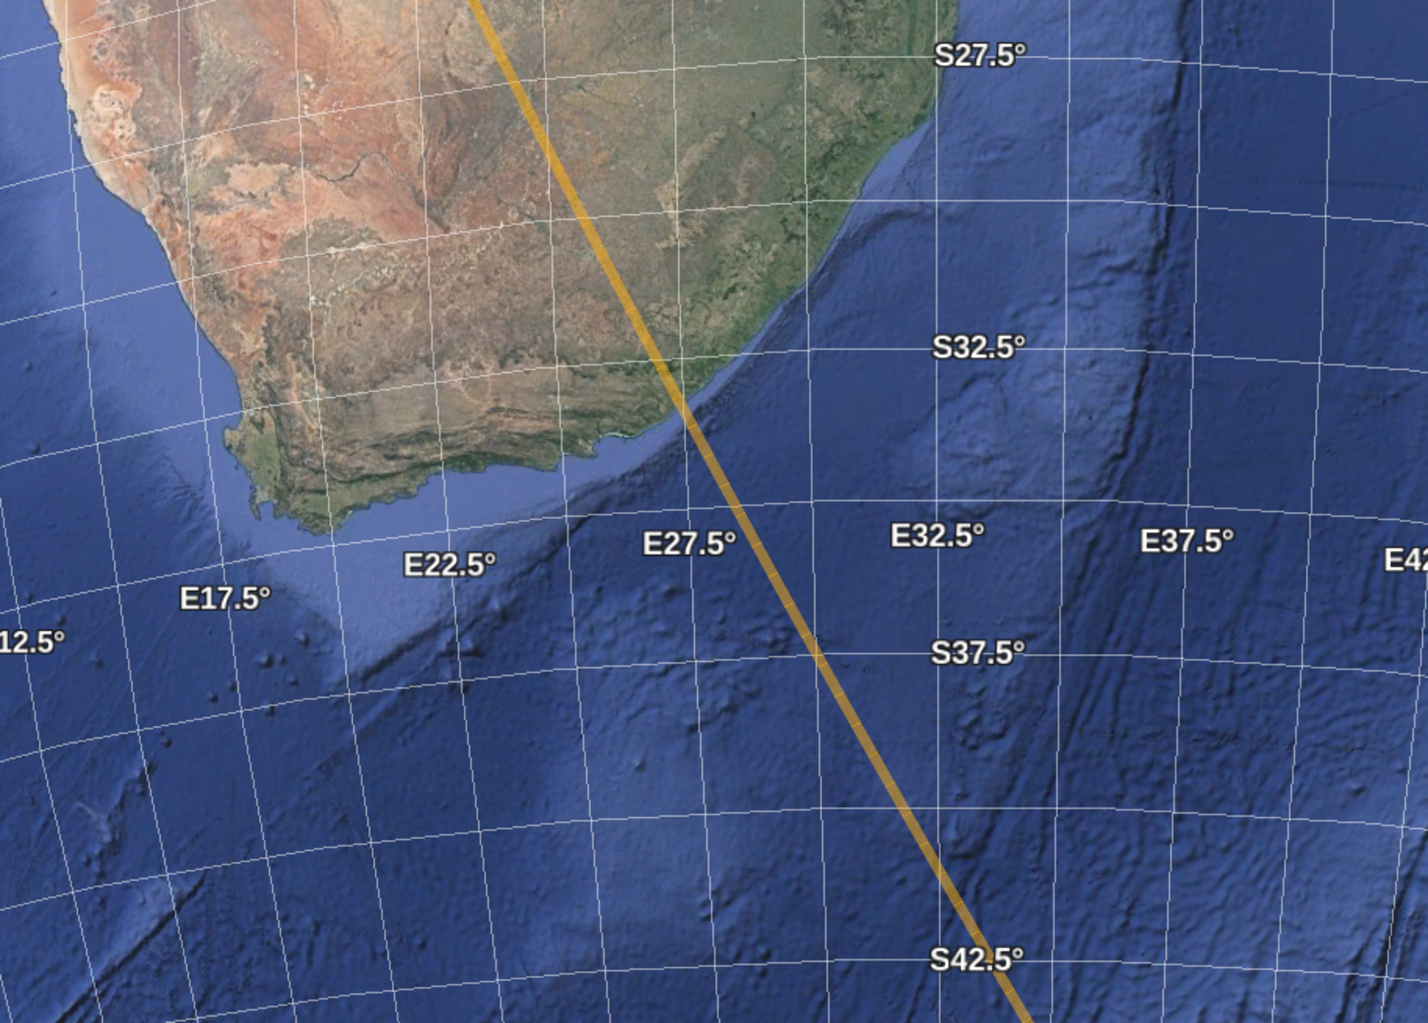
\includegraphics[width=0.7\textwidth]{fig/test_track}
\end{column}
\begin{column}{0.45\textwidth}\centering

\medskip
$\!\!\!\!\!$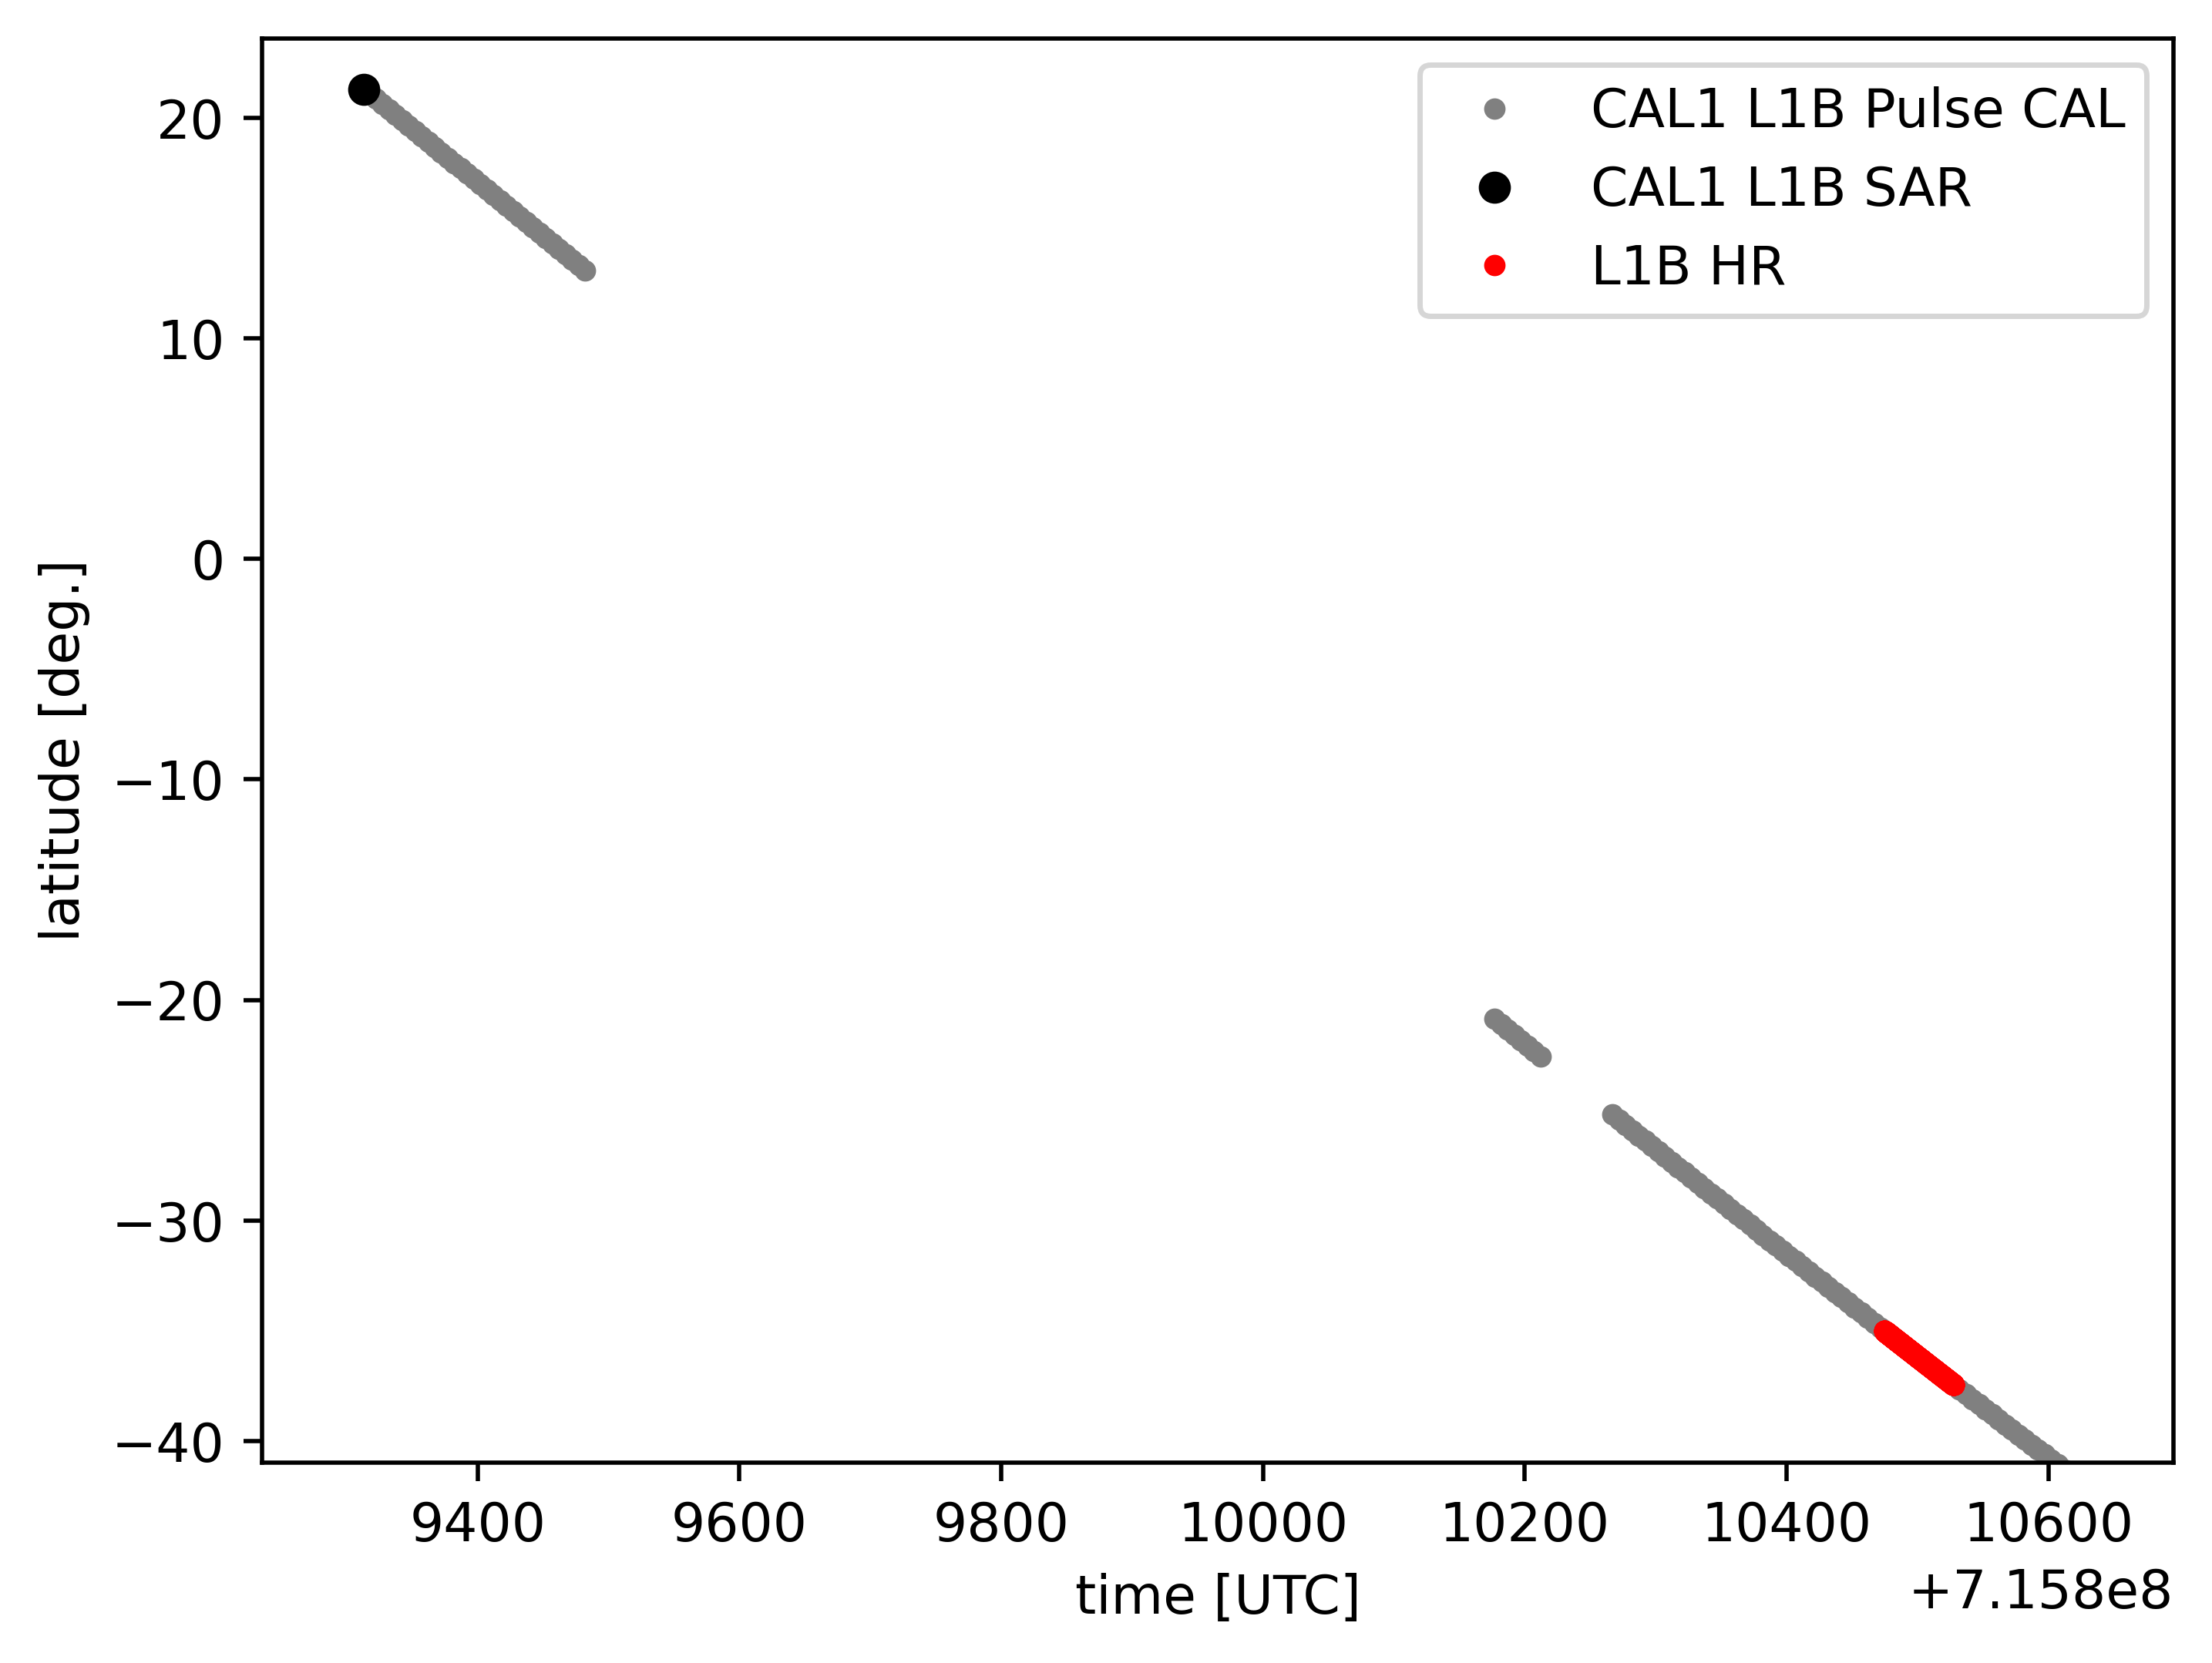
\includegraphics[width=0.78\textwidth]{fig/test_track_loc}
\end{column}
\end{columns}


\end{frame}



\section{Results and discussion}
\begin{frame}{Point target response in range (RIR)}
 
 
 \begin{figure}[htb!]
  \hspace{0.5cm} RIR CAL1 SAR \hspace{1.8cm} RIR CAL1 Pulse\hspace{1.8cm} RIR analytical
   
   \medskip
   \centering
  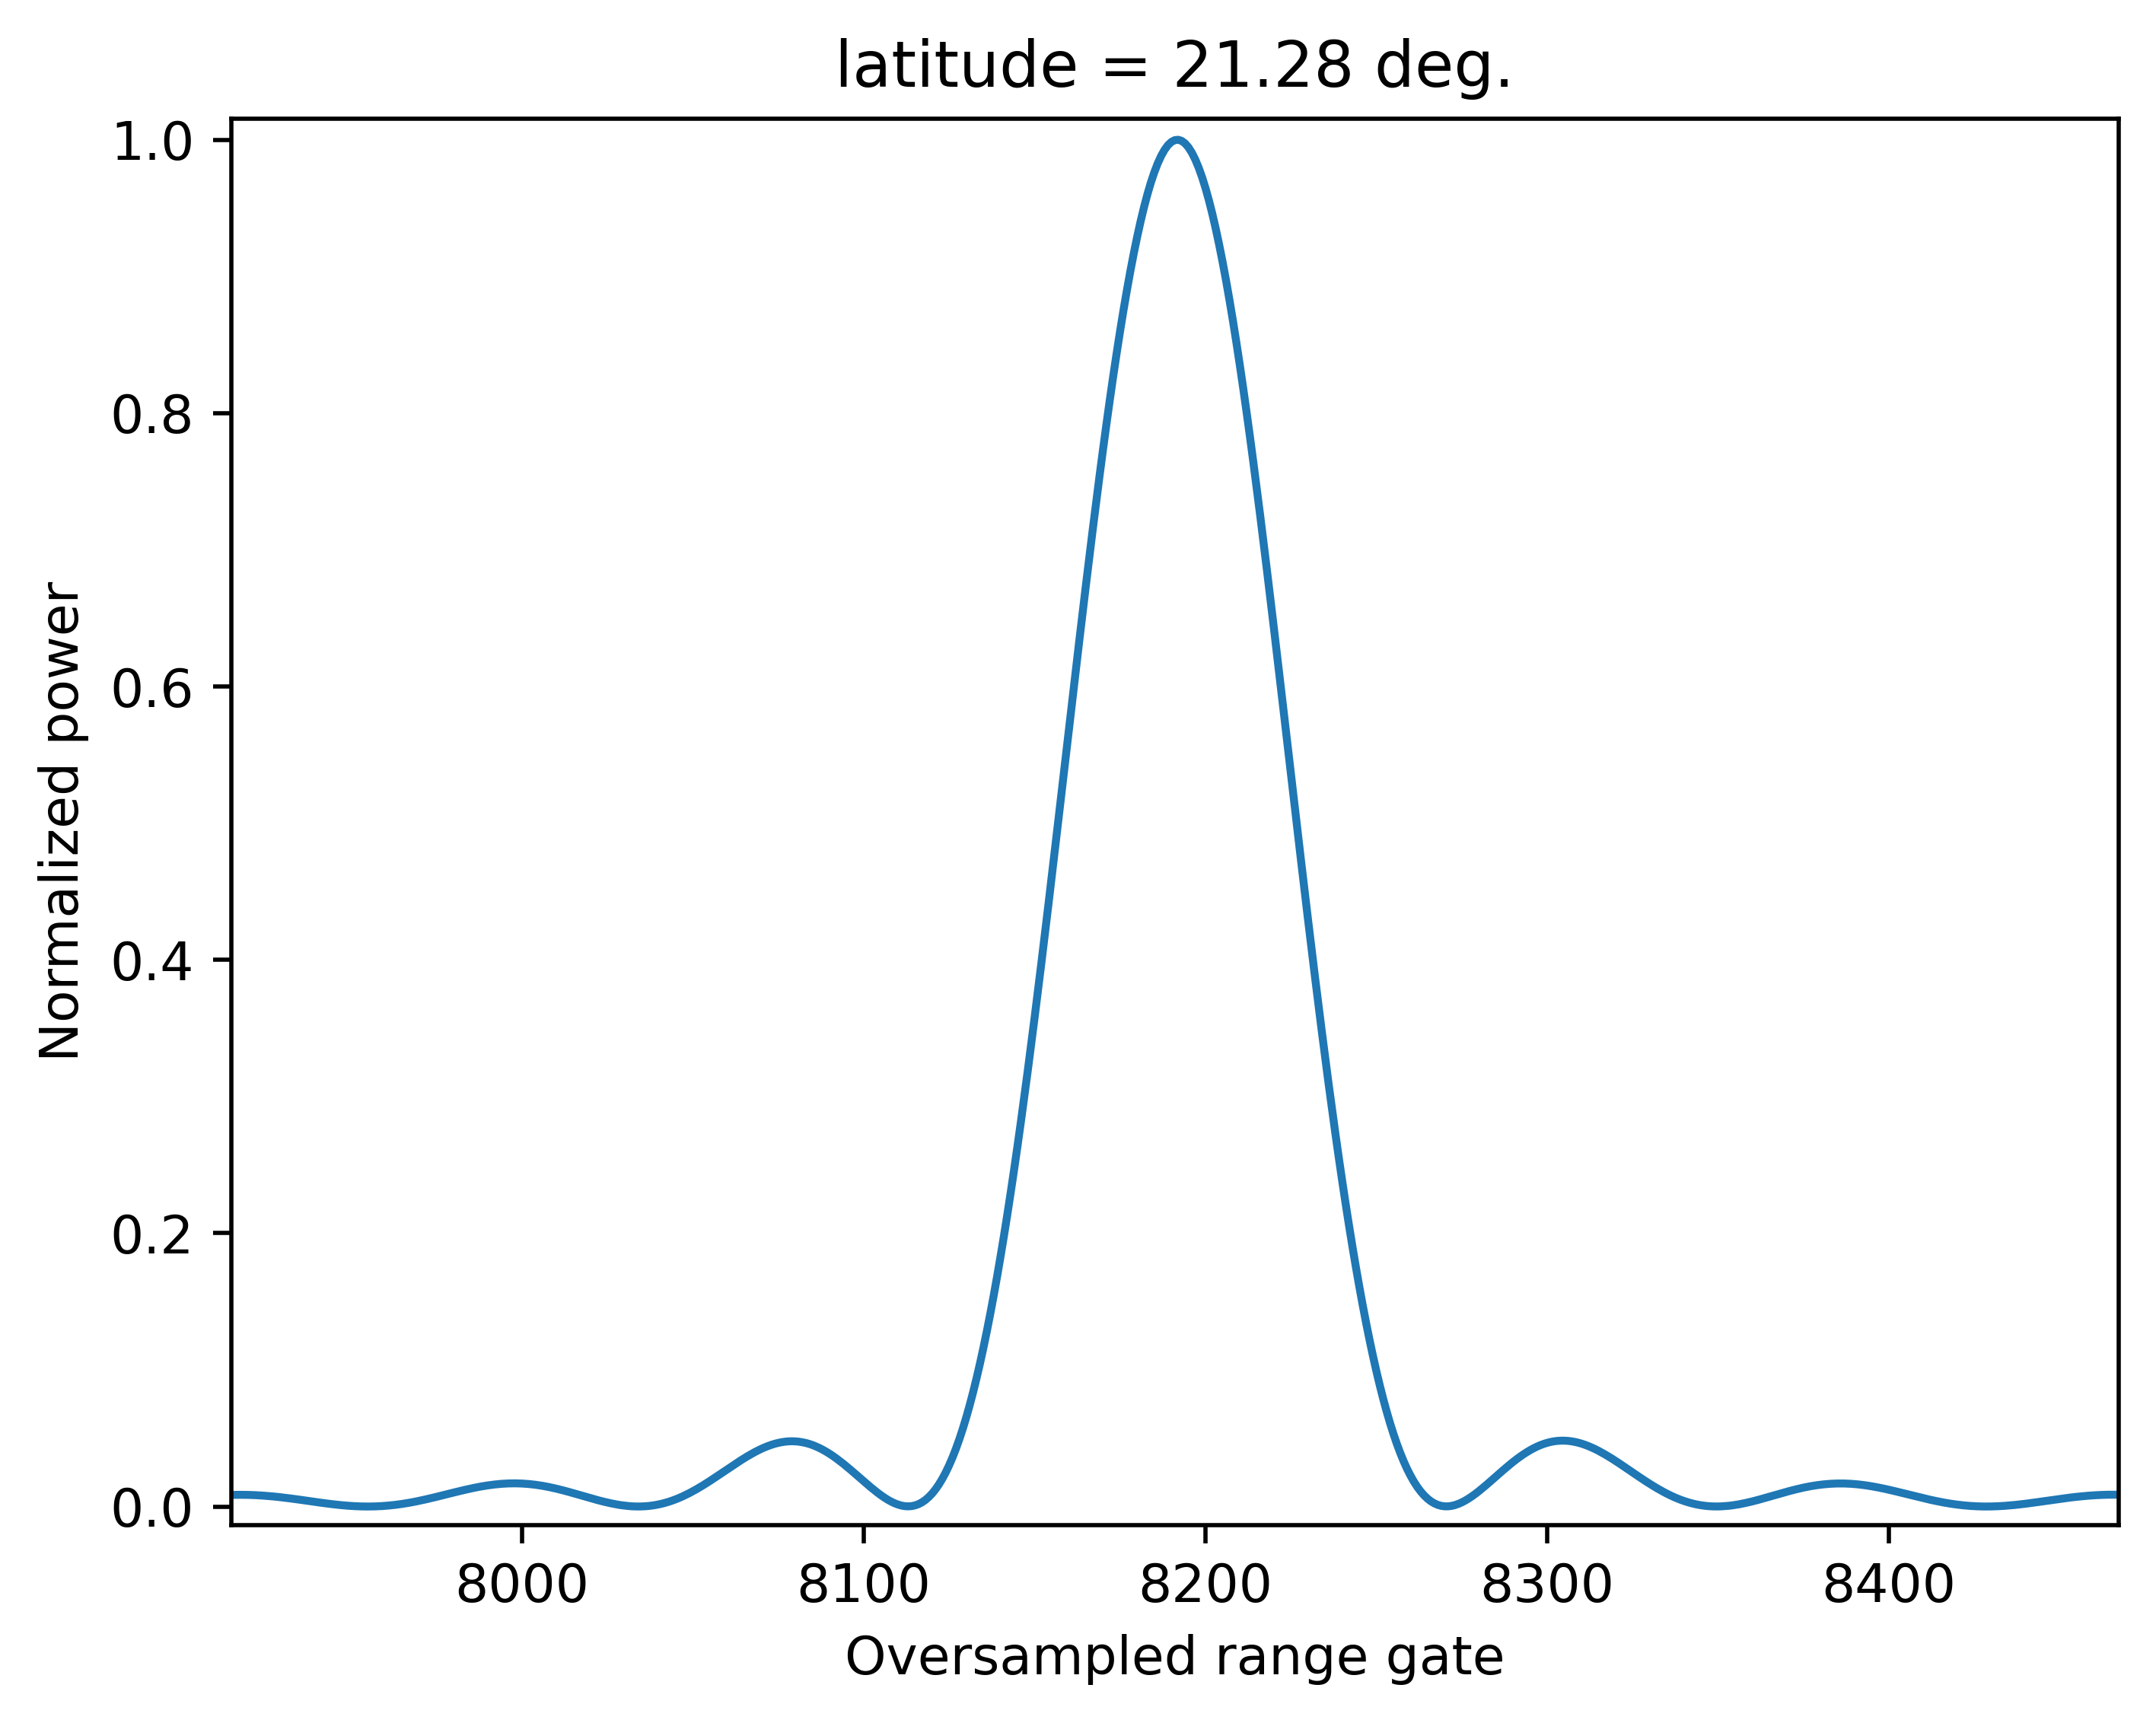
\includegraphics[width=0.32\textwidth]{fig/PTR_cal1sar}$\quad$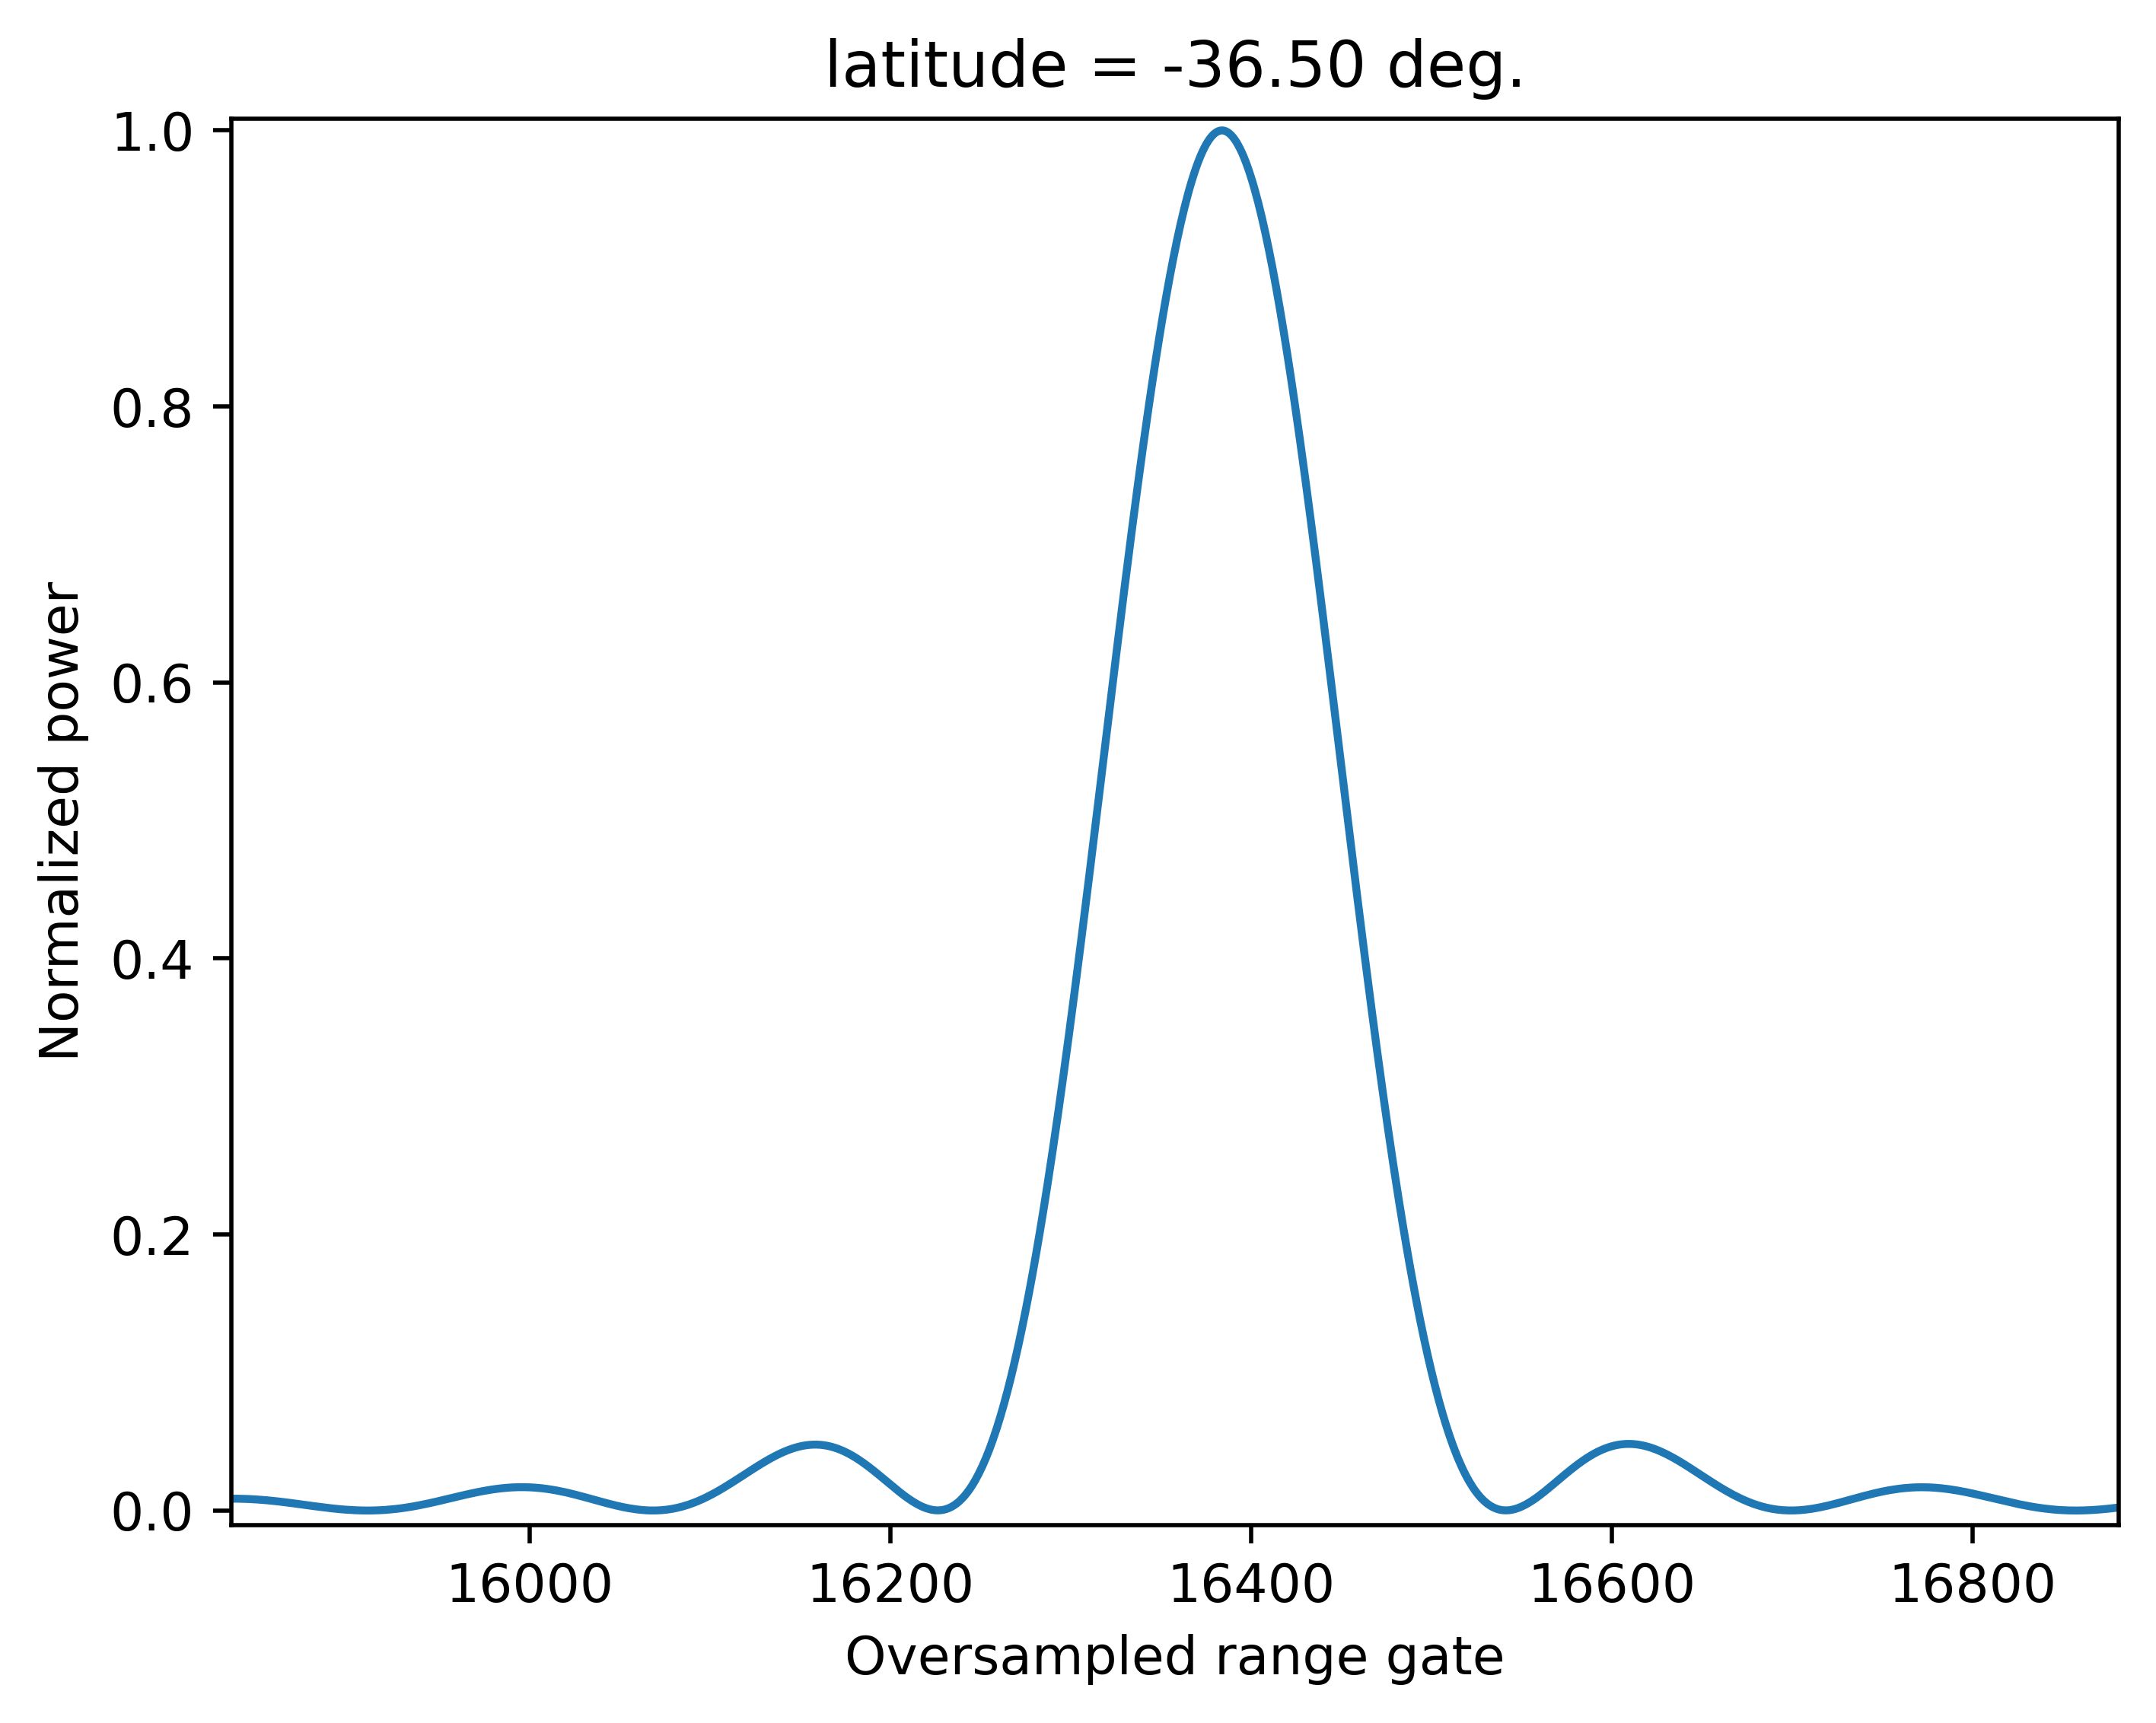
\includegraphics[width=0.32\textwidth]{fig/PTR_cal1pulse}$\quad$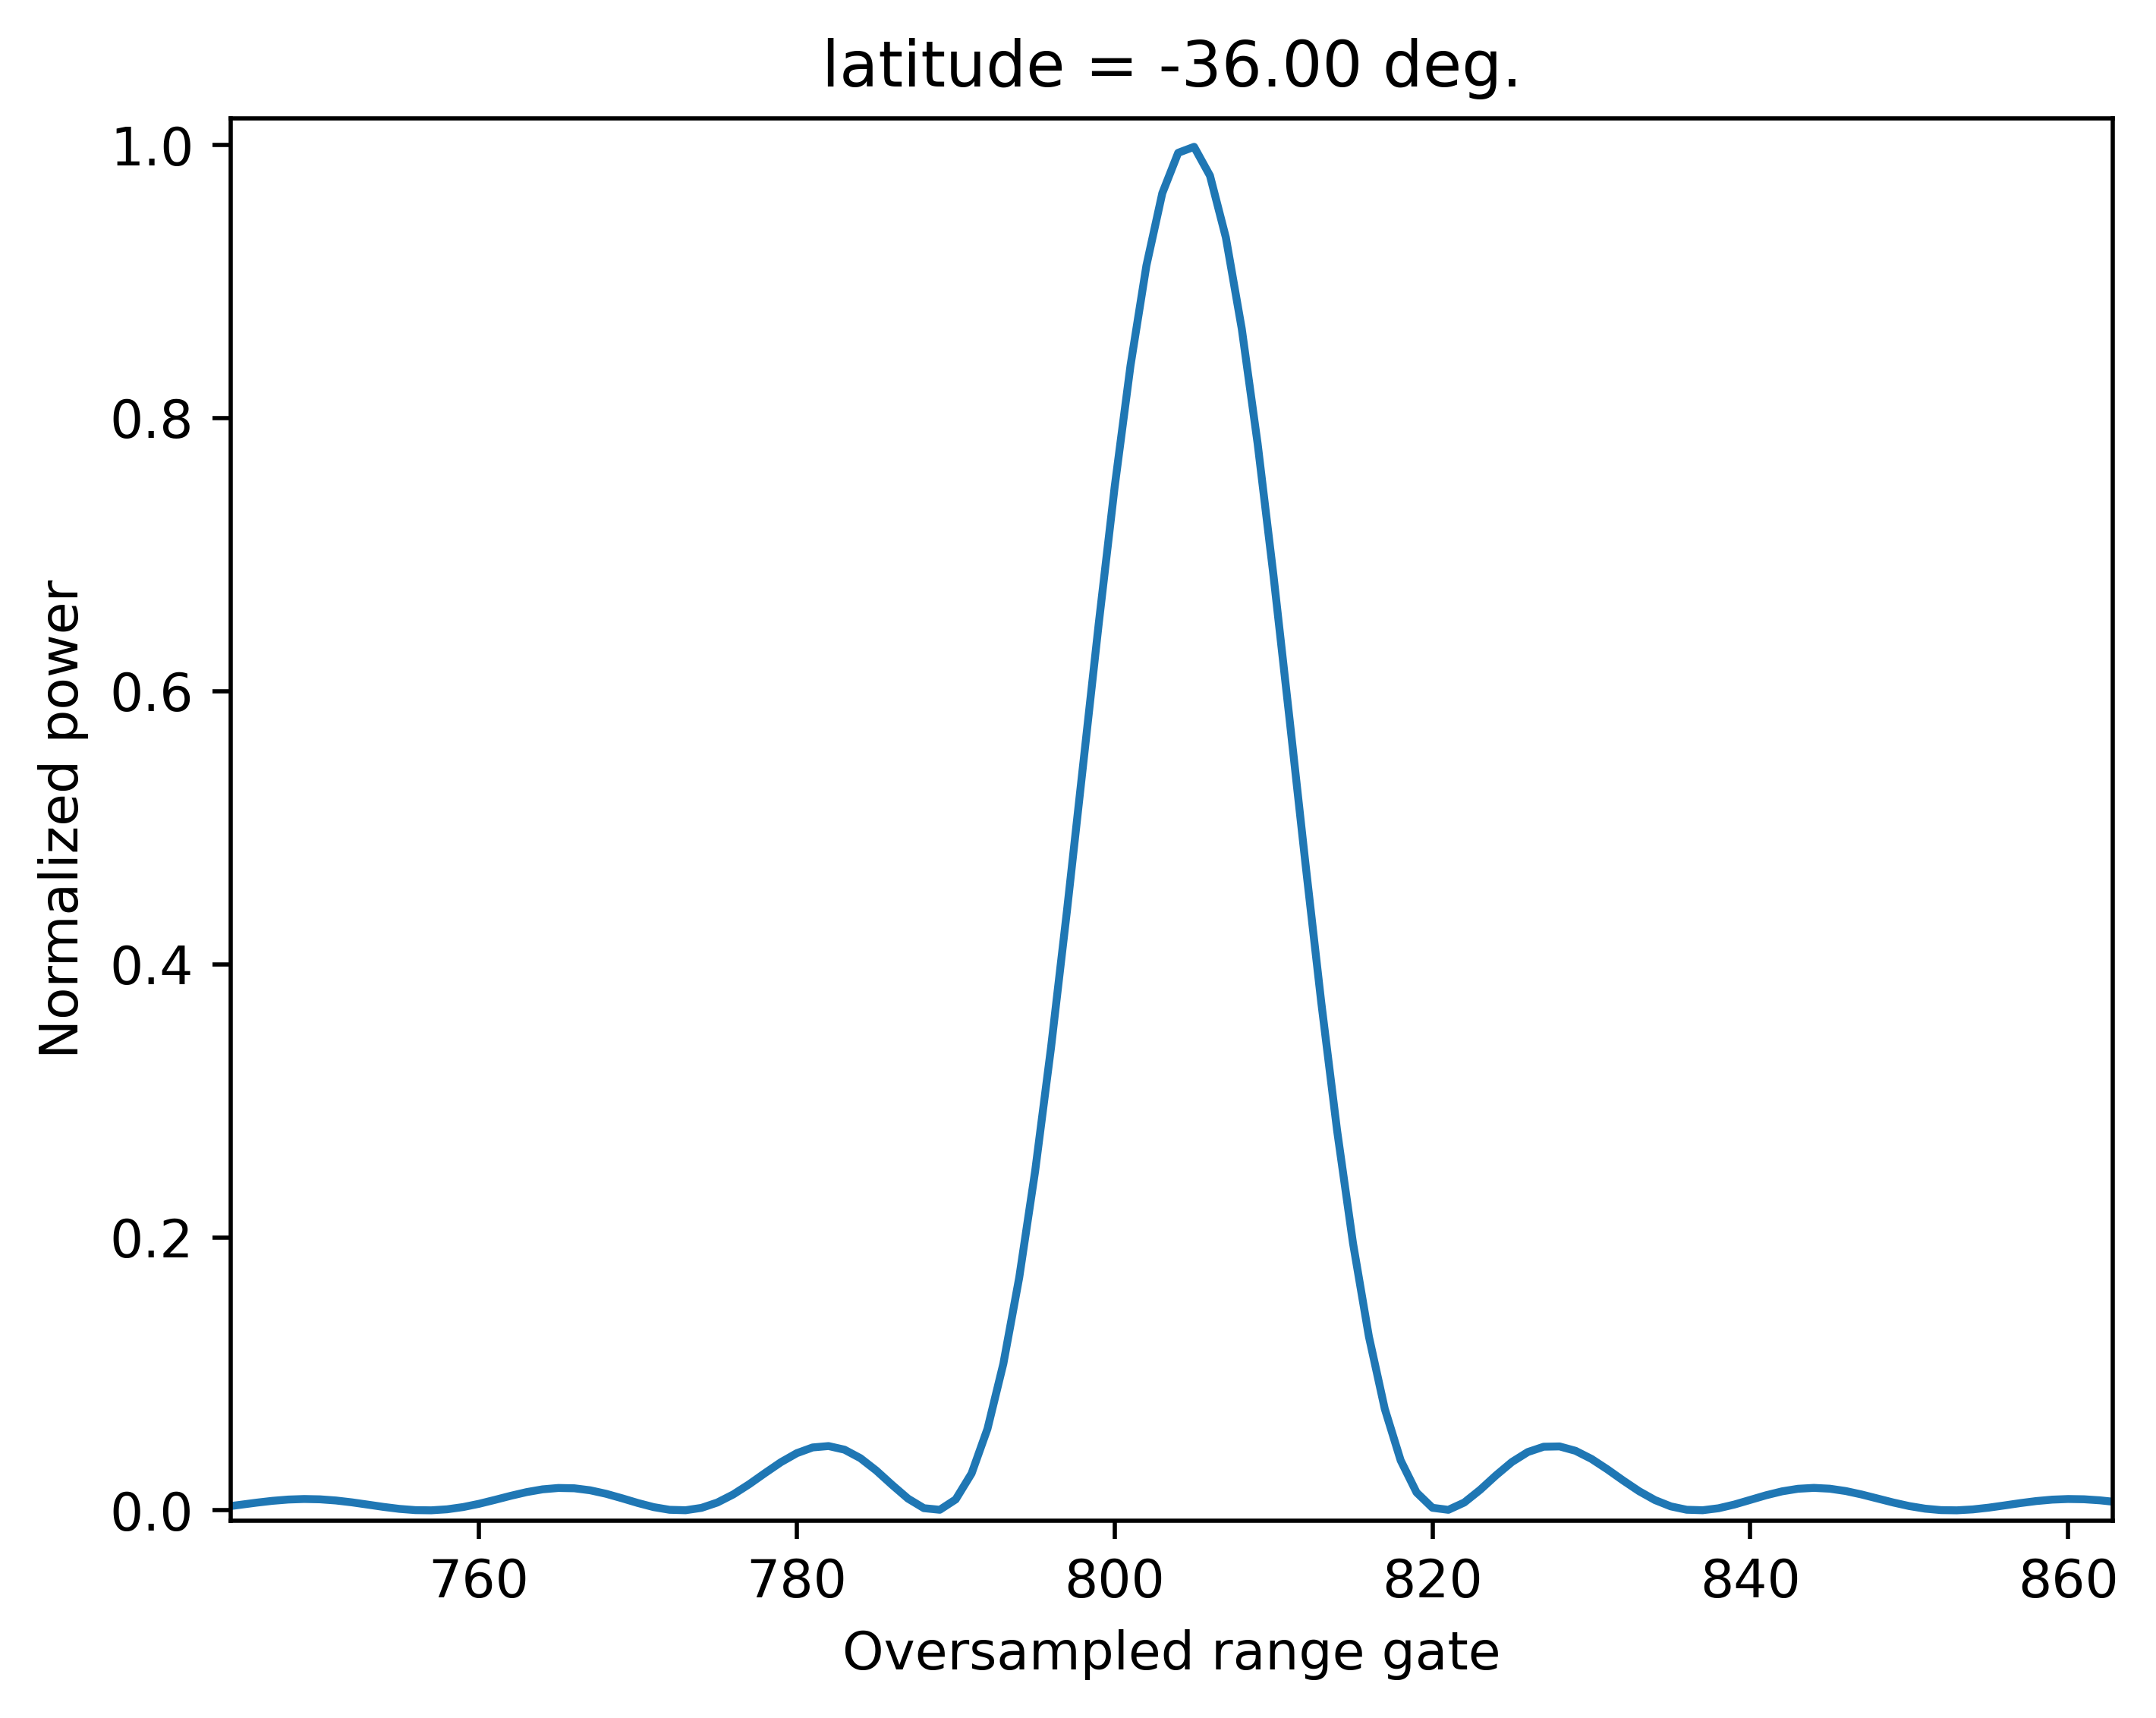
\includegraphics[width=0.32\textwidth]{fig/PTR_sinc}
\end{figure}

\begin{itemize}
 \item No apparent shape asymmetries of the PTR in range for this data.
  \item Strong similarities with analytical expression (sinc).
\end{itemize}


\end{frame}


\begin{frame}{Delay/Doppler model stack}

\medskip
\begin{columns}
\begin{column}{0.45\textwidth}\centering

Numerical (RIR CAL1 Pulse) before DC

  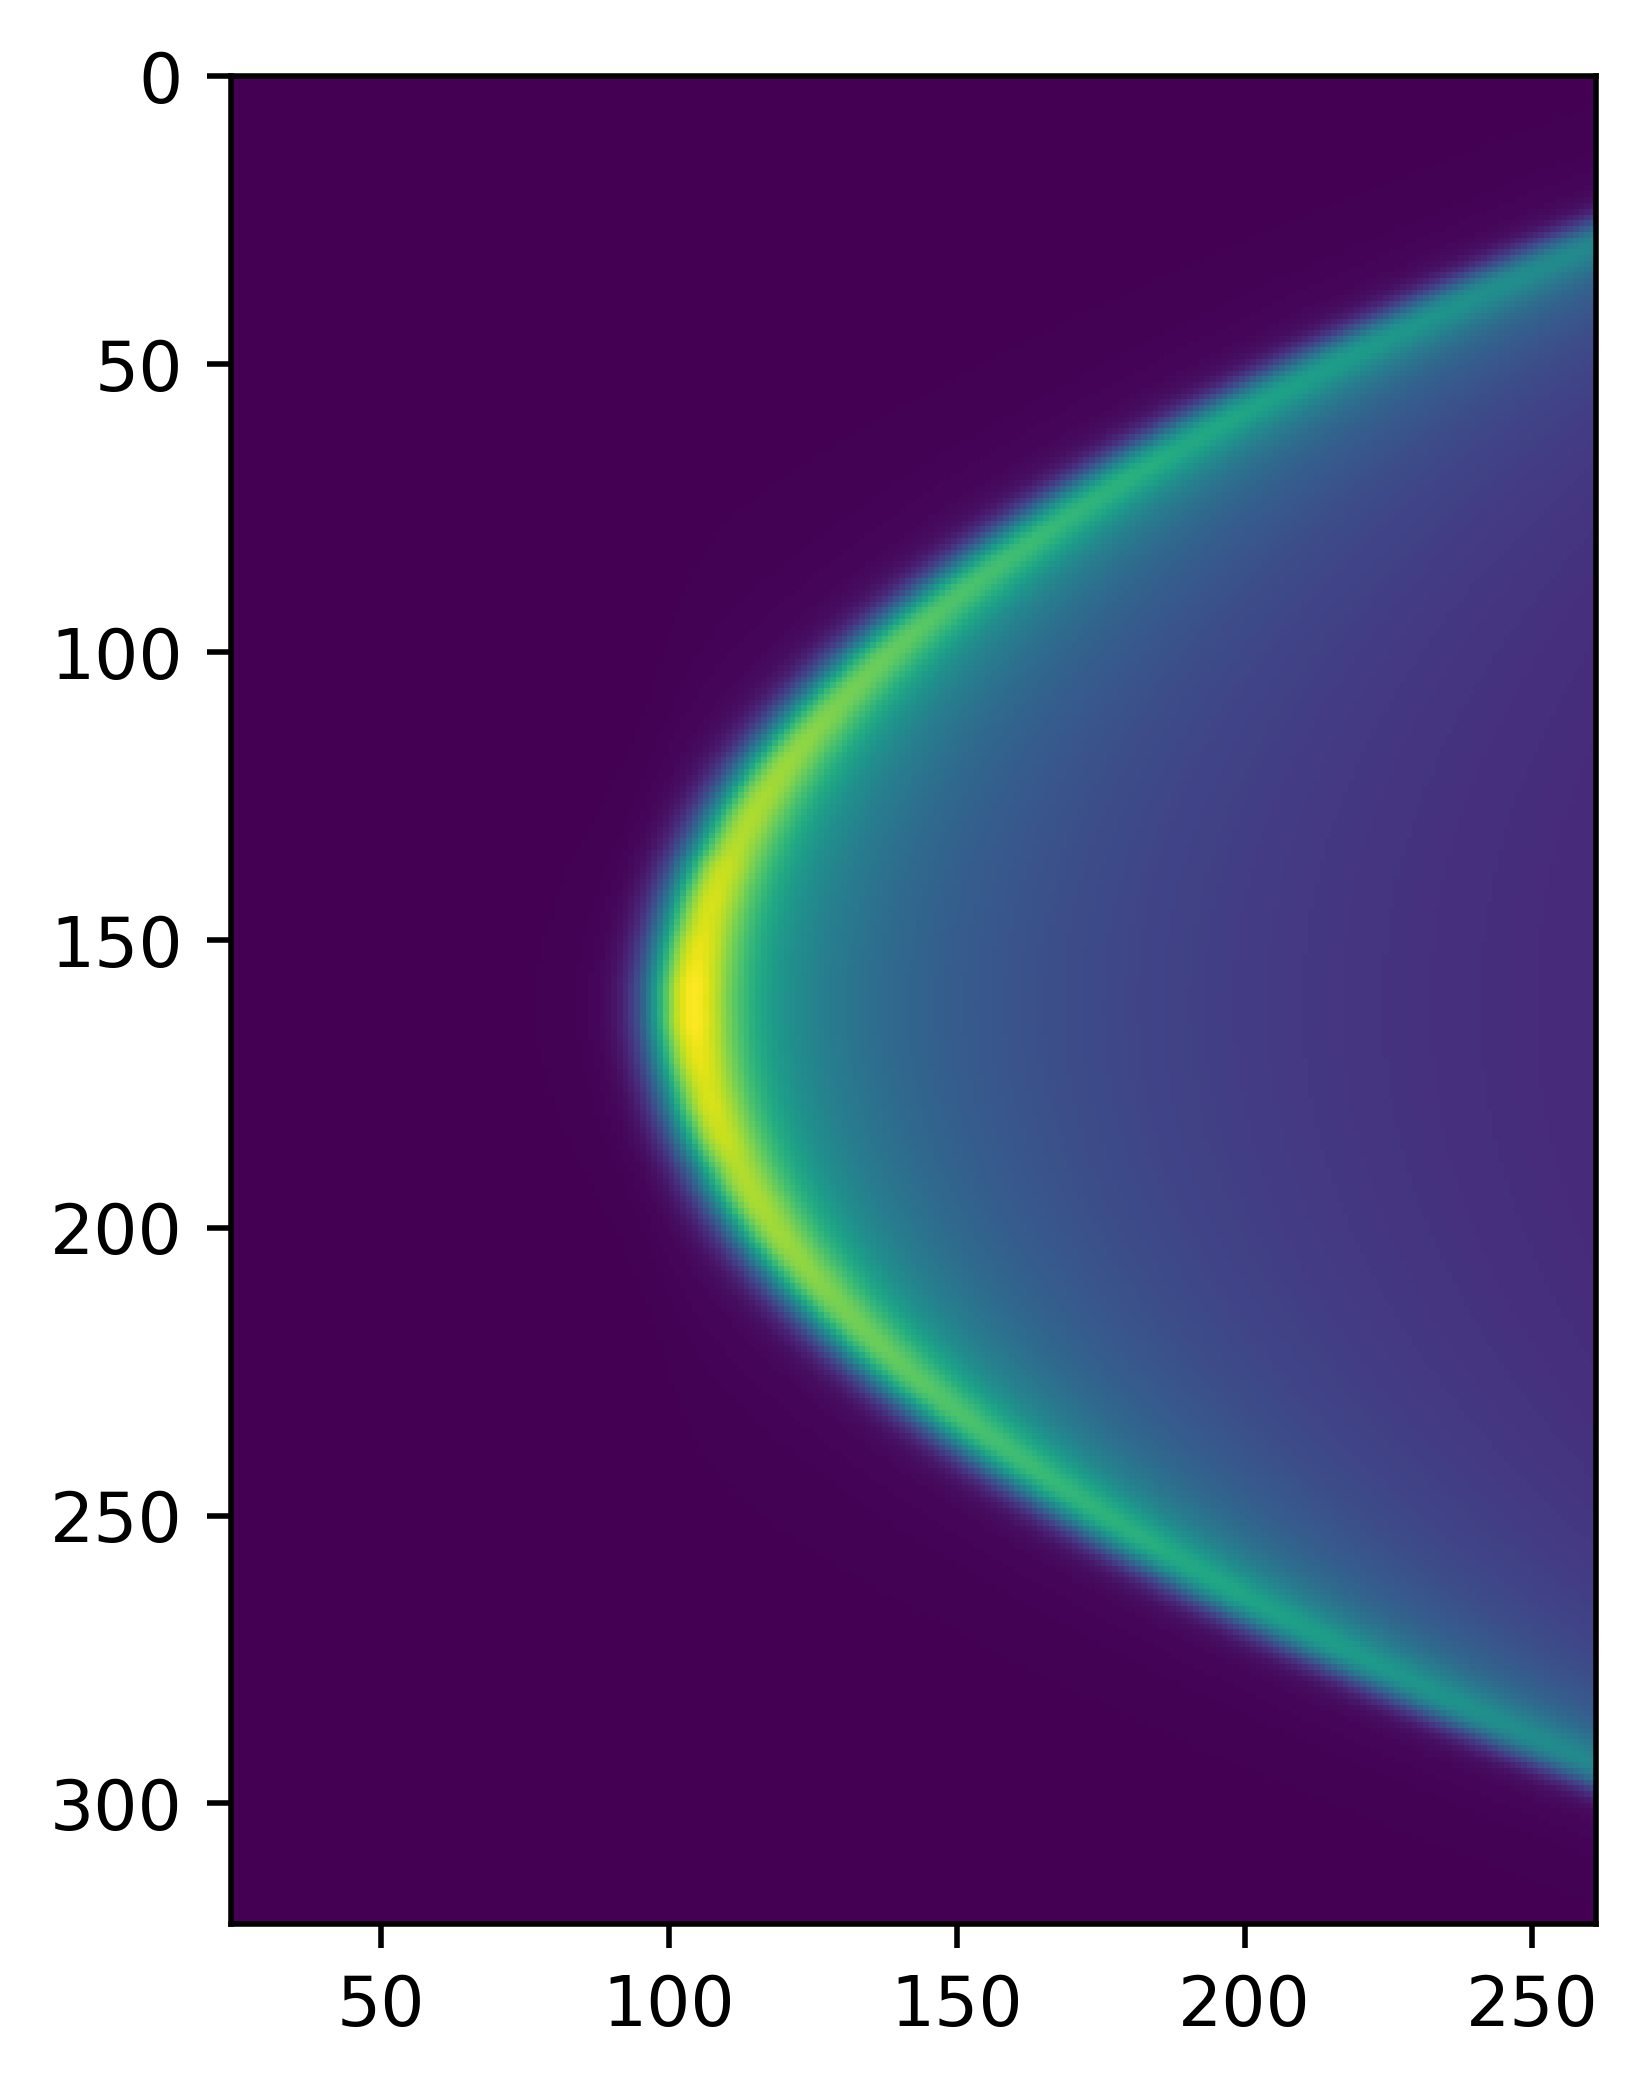
\includegraphics[width=0.45\textwidth]{fig/stack_num_PTRnum}

\end{column}
\begin{column}{0.45\textwidth}\centering

\begin{itemize}
 \item Delay compensation of power waveforms appears to align well the stack.
 \item Analytical retracker has delay compensation operation intrinsic in the closed-form expression.
 \item Different distribution of power along track between the two models.
\end{itemize}

  
\end{column}
\end{columns}
 
\begin{columns}
\begin{column}{0.45\textwidth}\centering

Numerical (RIR CAL1 Pulse) after DC

 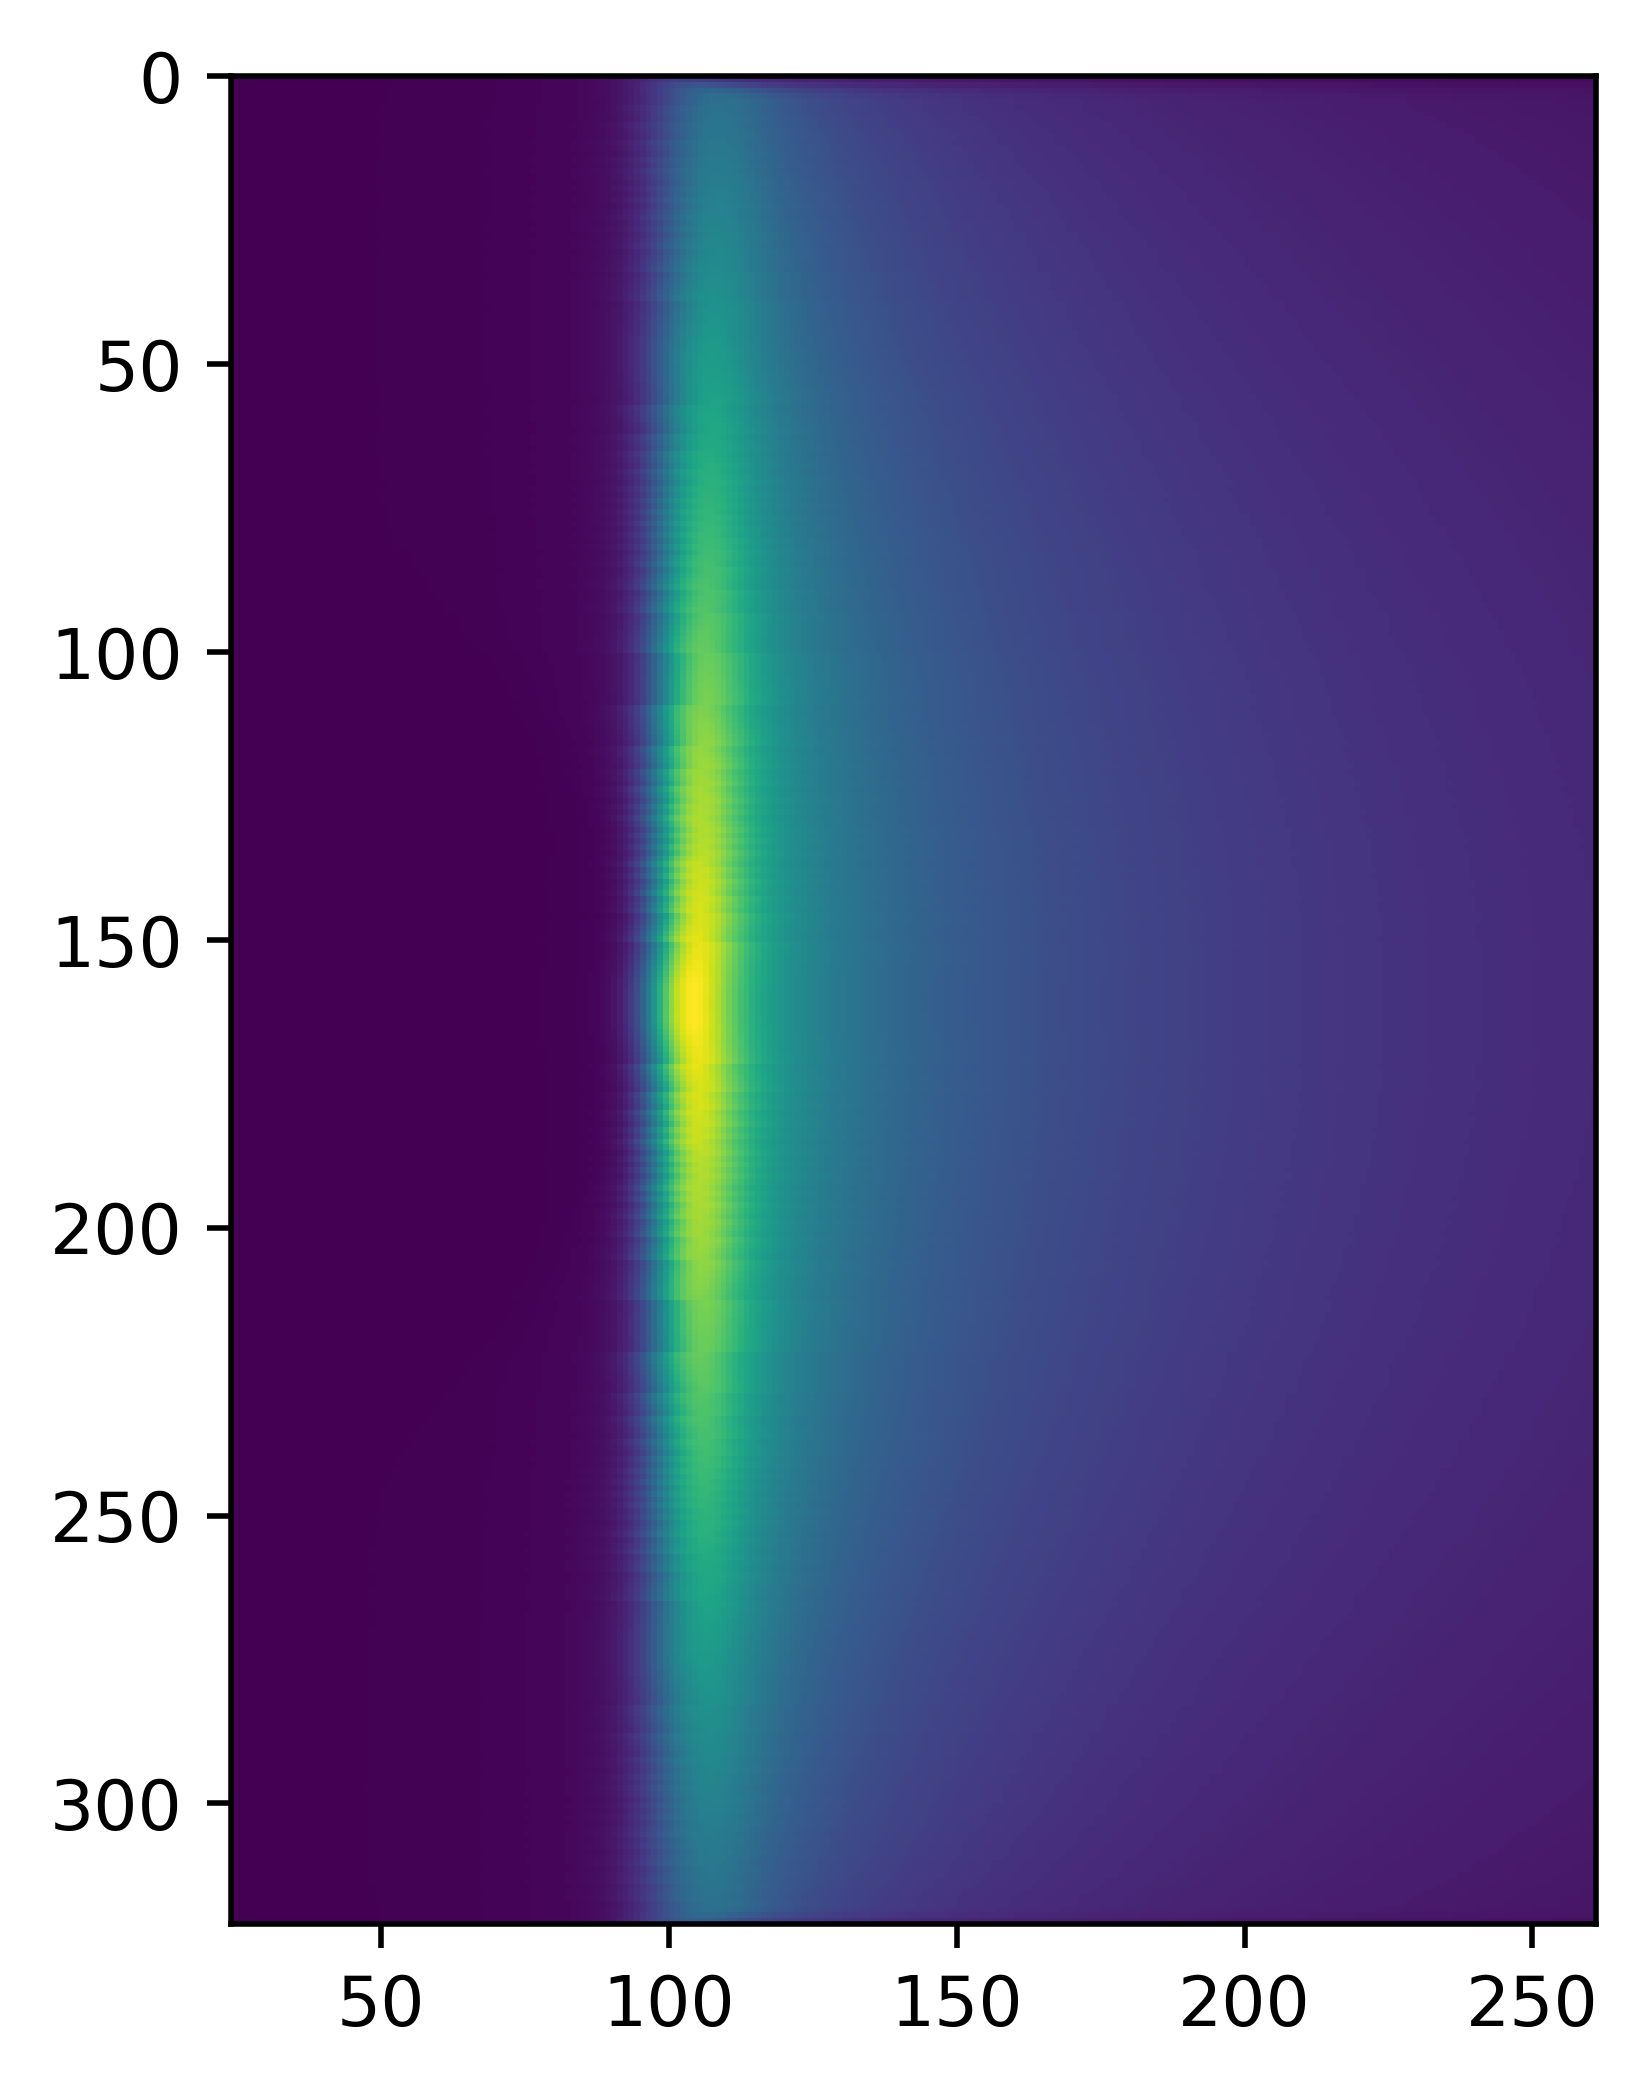
\includegraphics[width=0.45\textwidth]{fig/stack_dc_num_PTRnum}
\end{column}
\begin{column}{0.45\textwidth}\centering

Analytical retracker

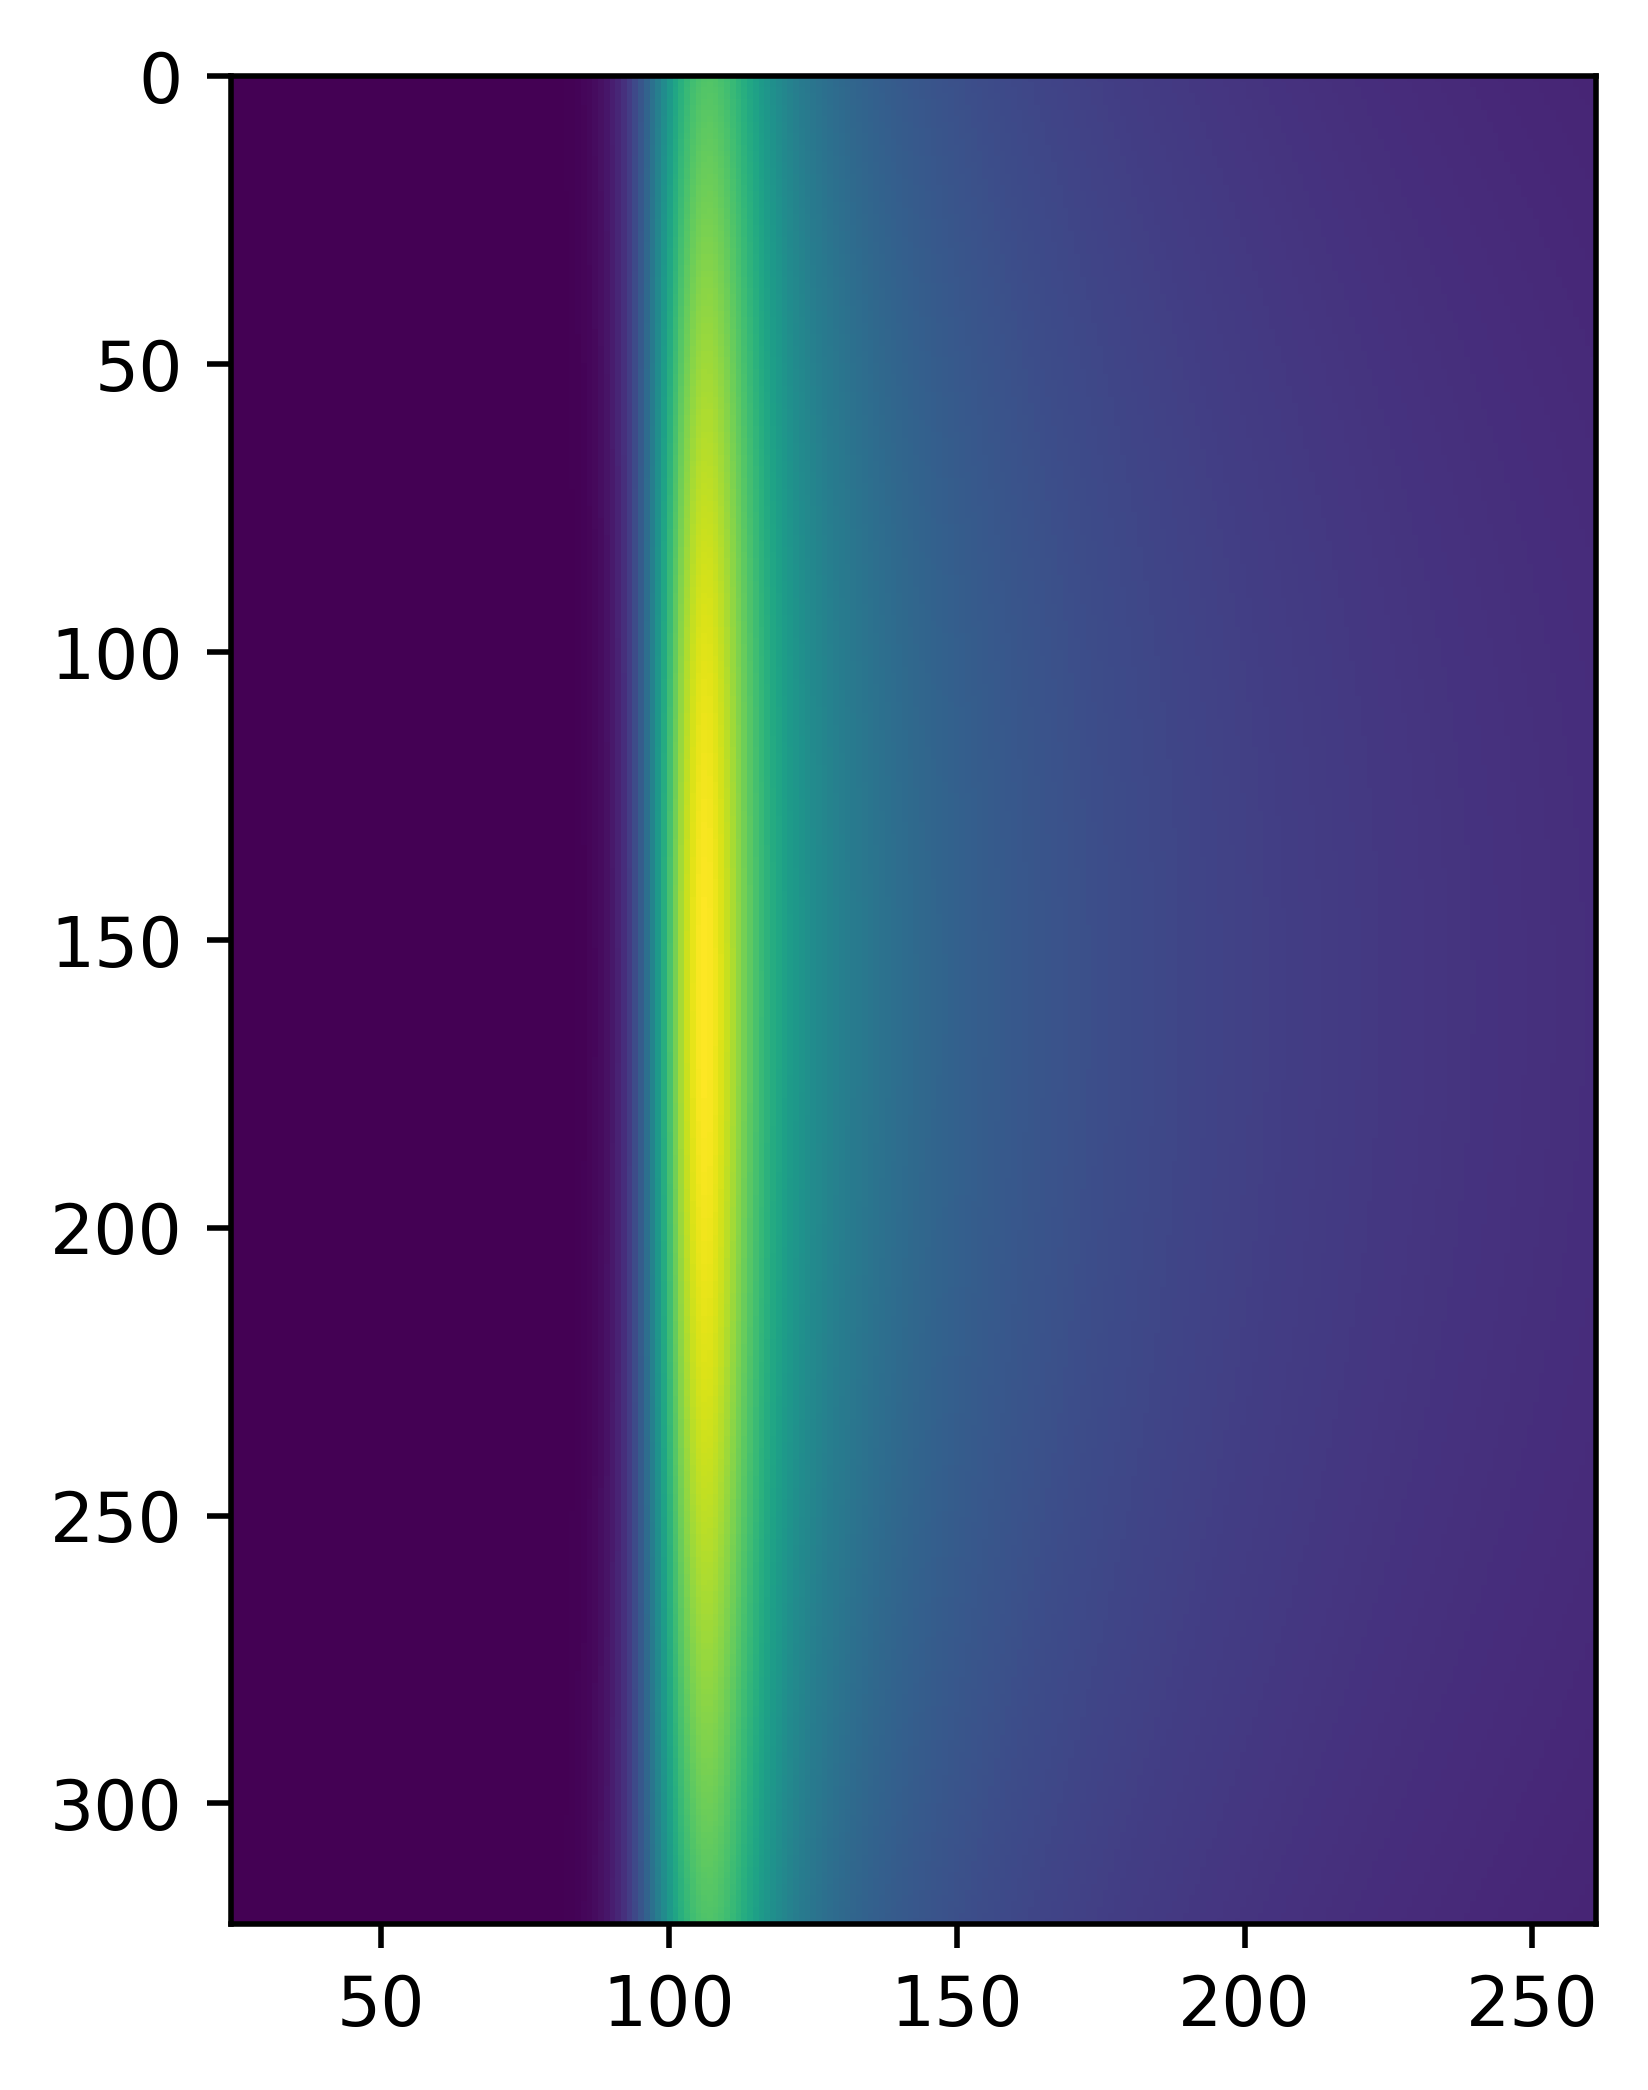
\includegraphics[width=0.45\textwidth]{fig/stack_dc_ana} 
  
\end{column}
\end{columns}

\end{frame}





\begin{frame}{Power waveforms after delay compensation and before multilooking}
 
 
 \begin{columns}
\begin{column}{0.45\textwidth}\centering

Numerical (RIR CAL1 Pulse)

  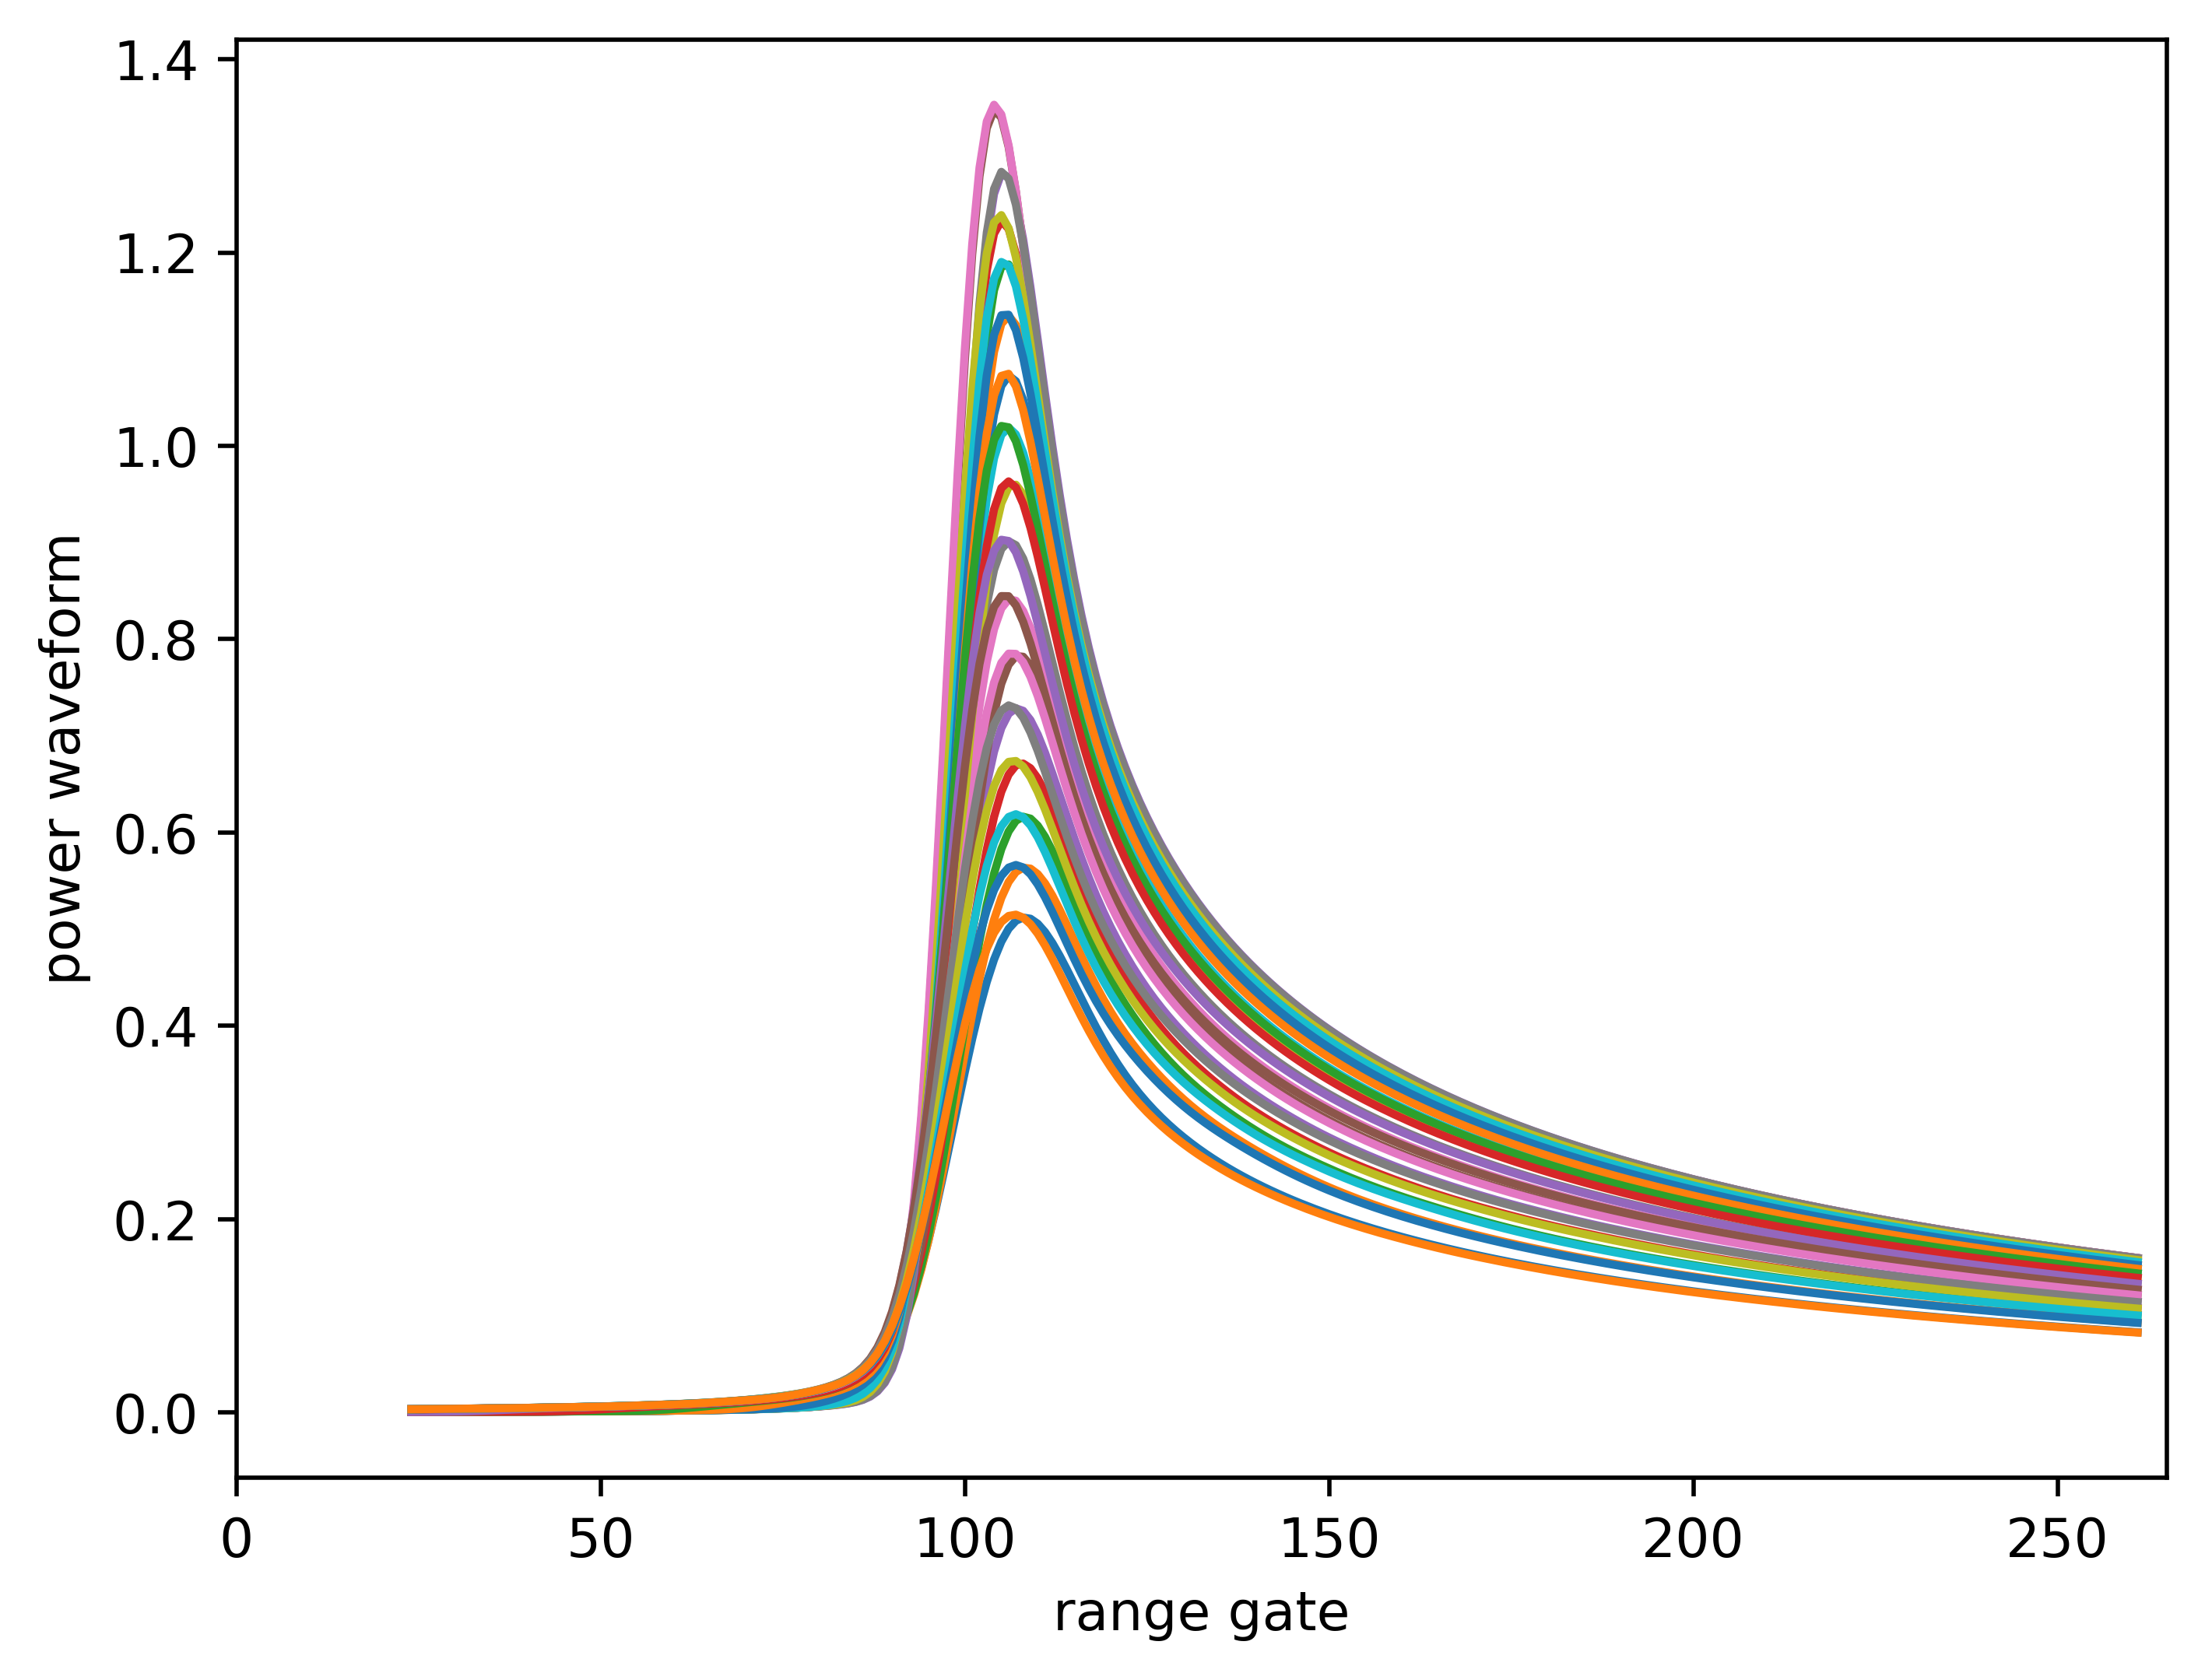
\includegraphics[width=0.9\textwidth]{fig/waveforms_dc_num_PTRnum}

\end{column}
\begin{column}{0.45\textwidth}\centering

Analytical retracker

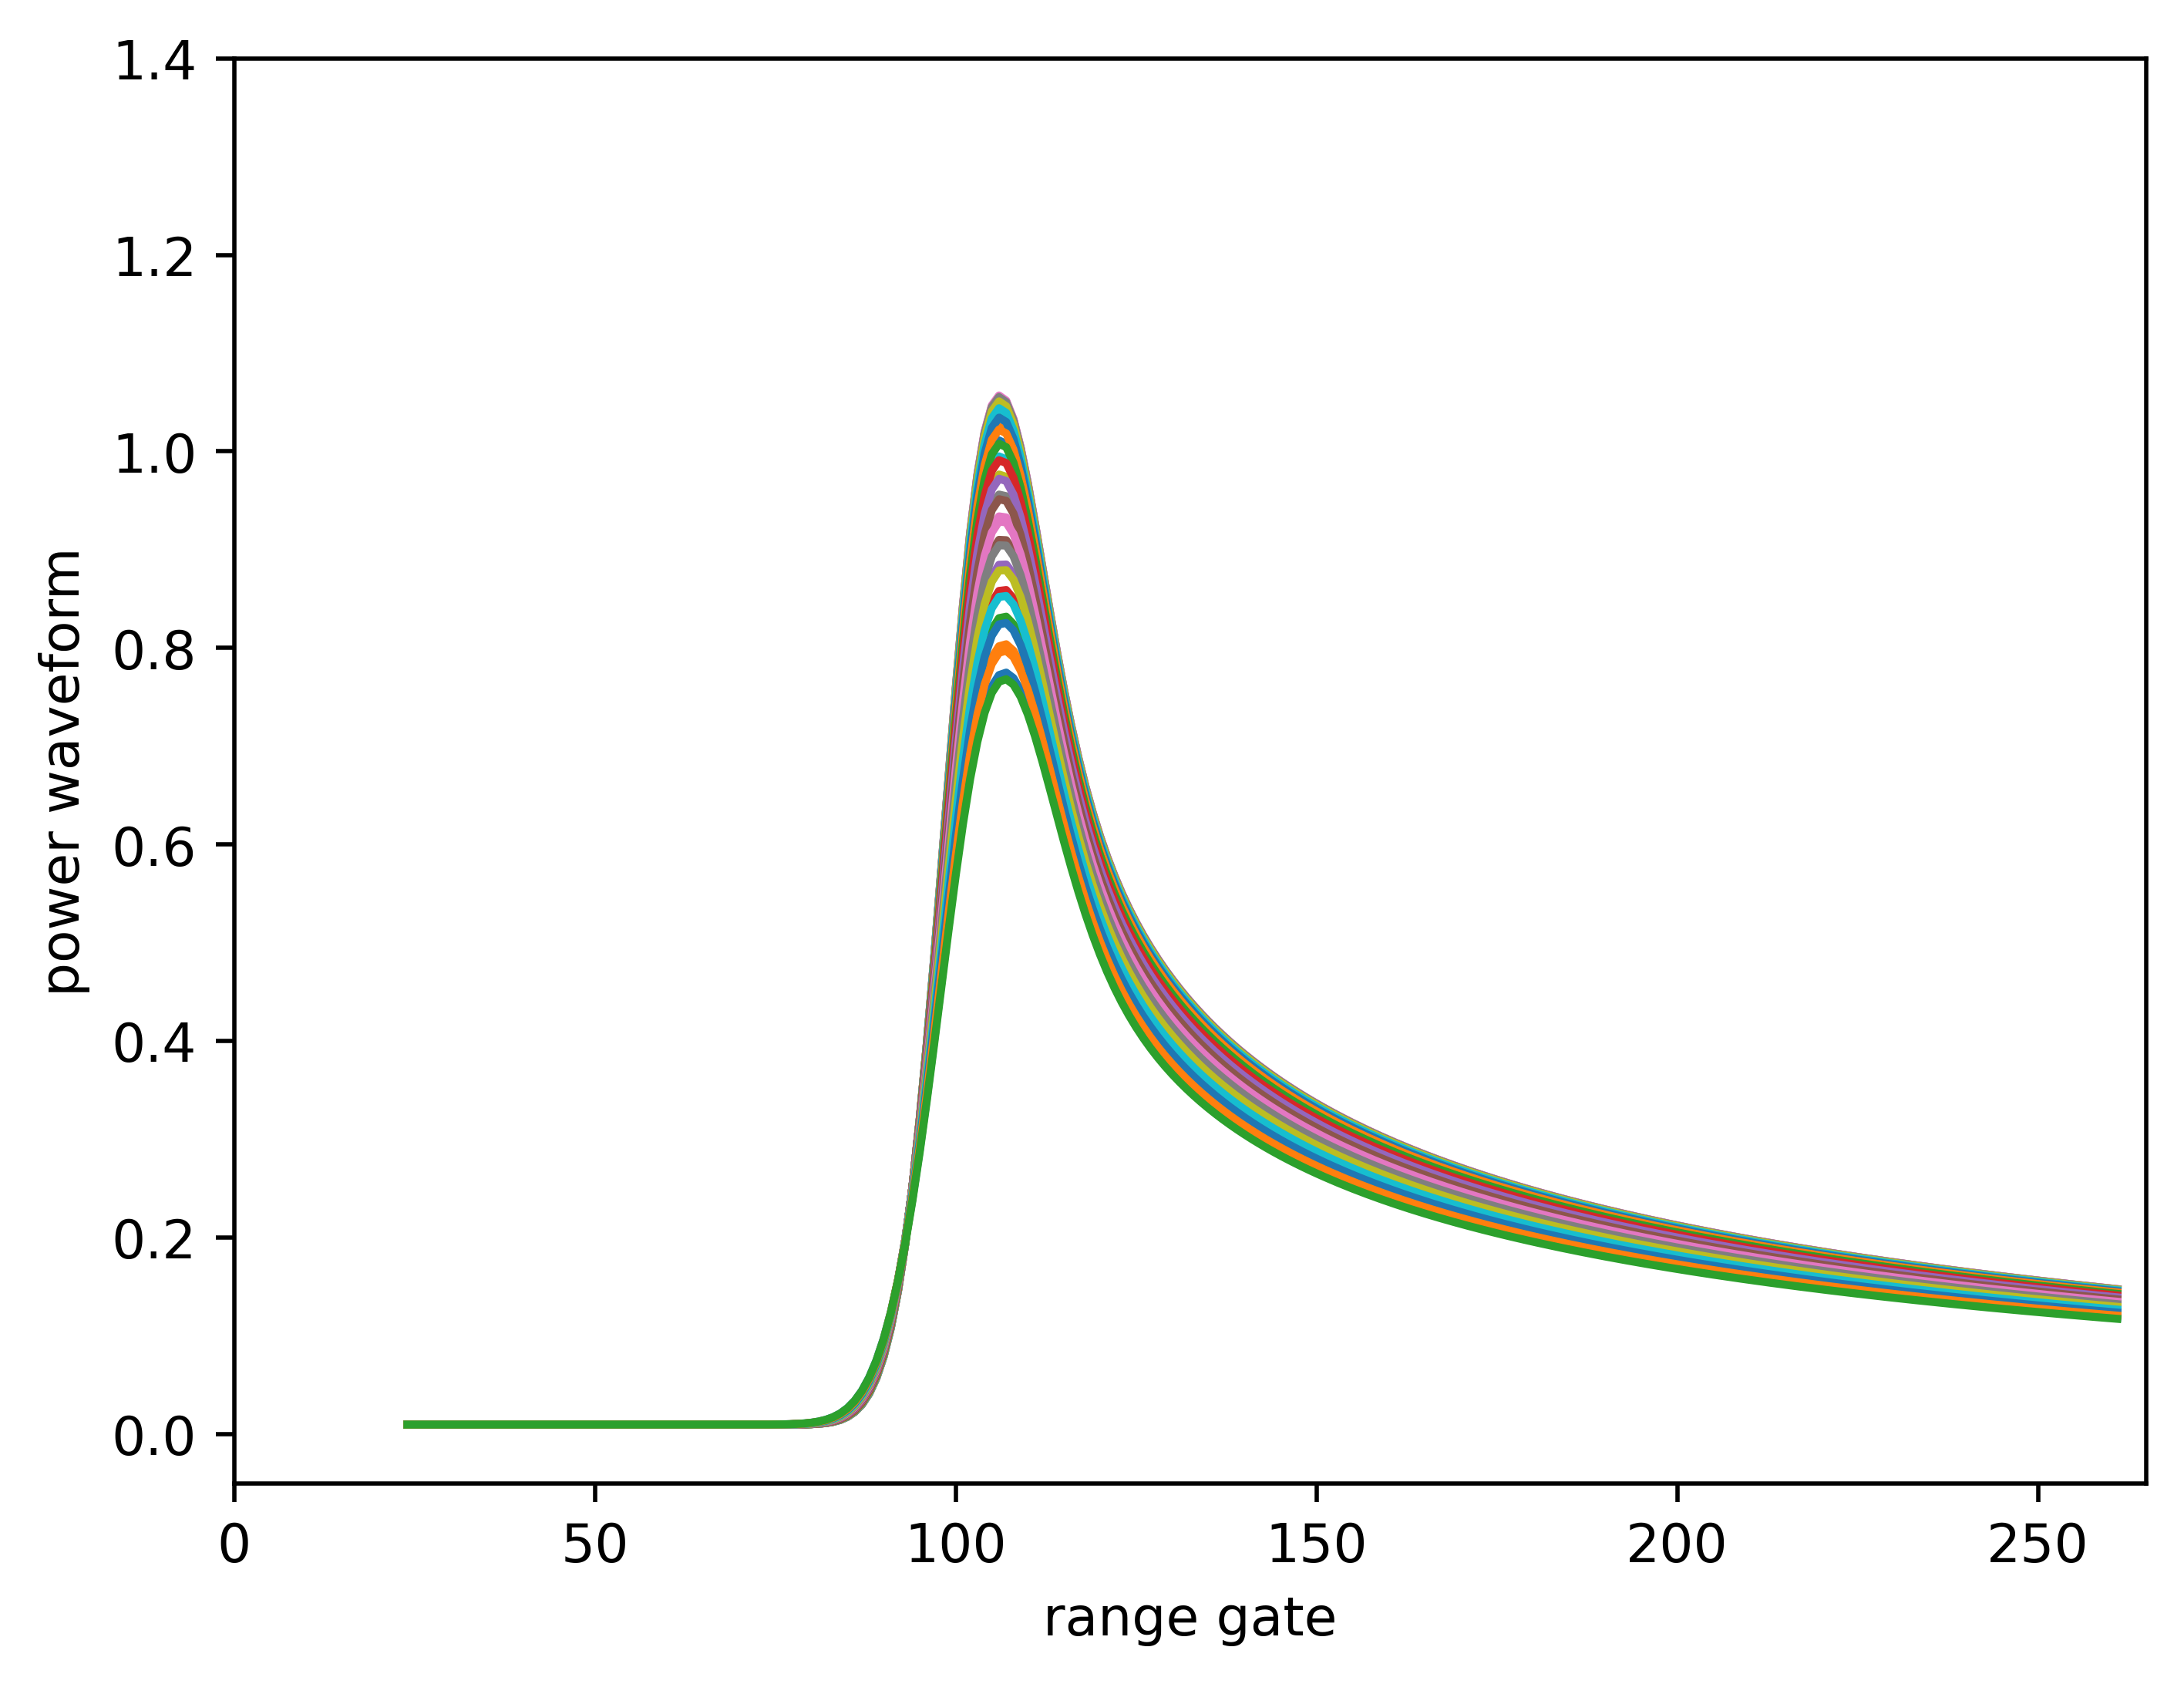
\includegraphics[width=0.9\textwidth]{fig/waveforms_dc_ana_PTRana} 
  
\end{column}
\end{columns}

\vspace{1cm}
\begin{itemize}
 \item A subset of waveforms along the beams are illustrated for simplicity.
 \item Power distributed differently along the beams in both retrackers.
\end{itemize}

\end{frame}





\begin{frame}{Multilooked waveforms}
 
 
 \begin{columns}
\begin{column}{0.45\textwidth}\centering

Numerical (RIR CAL1 Pulse)

  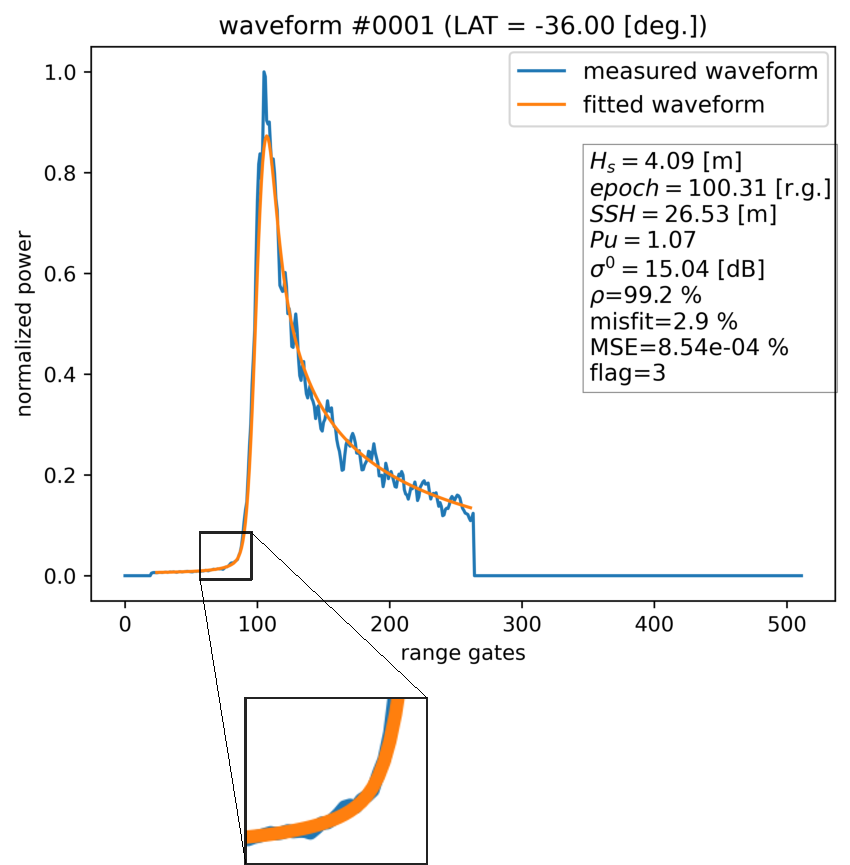
\includegraphics[width=0.9\textwidth]{fig/wfm_1_num_PTRnum_zoom}

\end{column}
\begin{column}{0.45\textwidth}\centering

Analytical retracker

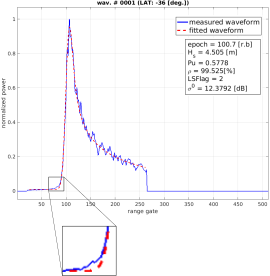
\includegraphics[width=0.9\textwidth]{fig/wfm_1_ana} 
  
\end{column}
\end{columns}

\begin{itemize}
 \item Perfect fit of the waveform's toe.
 \item Pearson correlation coefficients $\rho$ between model and measurement $> 99\%$.
\end{itemize}

\end{frame}



\begin{frame}{Multilooked waveforms}
 
 
 \begin{columns}
\begin{column}{0.45\textwidth}\centering

Numerical (RIR CAL1 Pulse)

  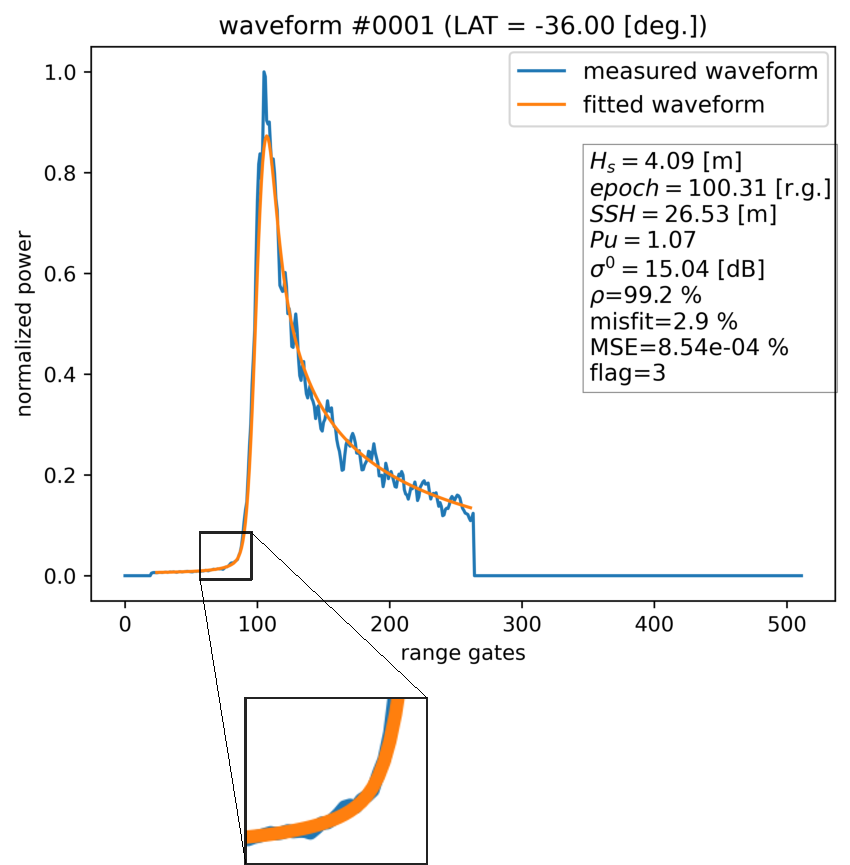
\includegraphics[width=0.9\textwidth]{fig/wfm_1_num_PTRnum_zoom}

\end{column}
\begin{column}{0.45\textwidth}\centering

Numerical (RIR analytical)

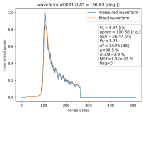
\includegraphics[width=0.9\textwidth]{fig/wfm_1_num_PTRana_zoom} 
  
\end{column}
\end{columns}

\begin{itemize}
 \item Numerical retracker with analytical RIR (right) appears to slightly worsen the fitting ($\rho$).
 
 .
\end{itemize}

\end{frame}






\begin{frame}{Effect of oversampling \textnormal{- default: azimuth $10$, range $8$}}


 \begin{columns}
\begin{column}{0.45\textwidth}\centering

  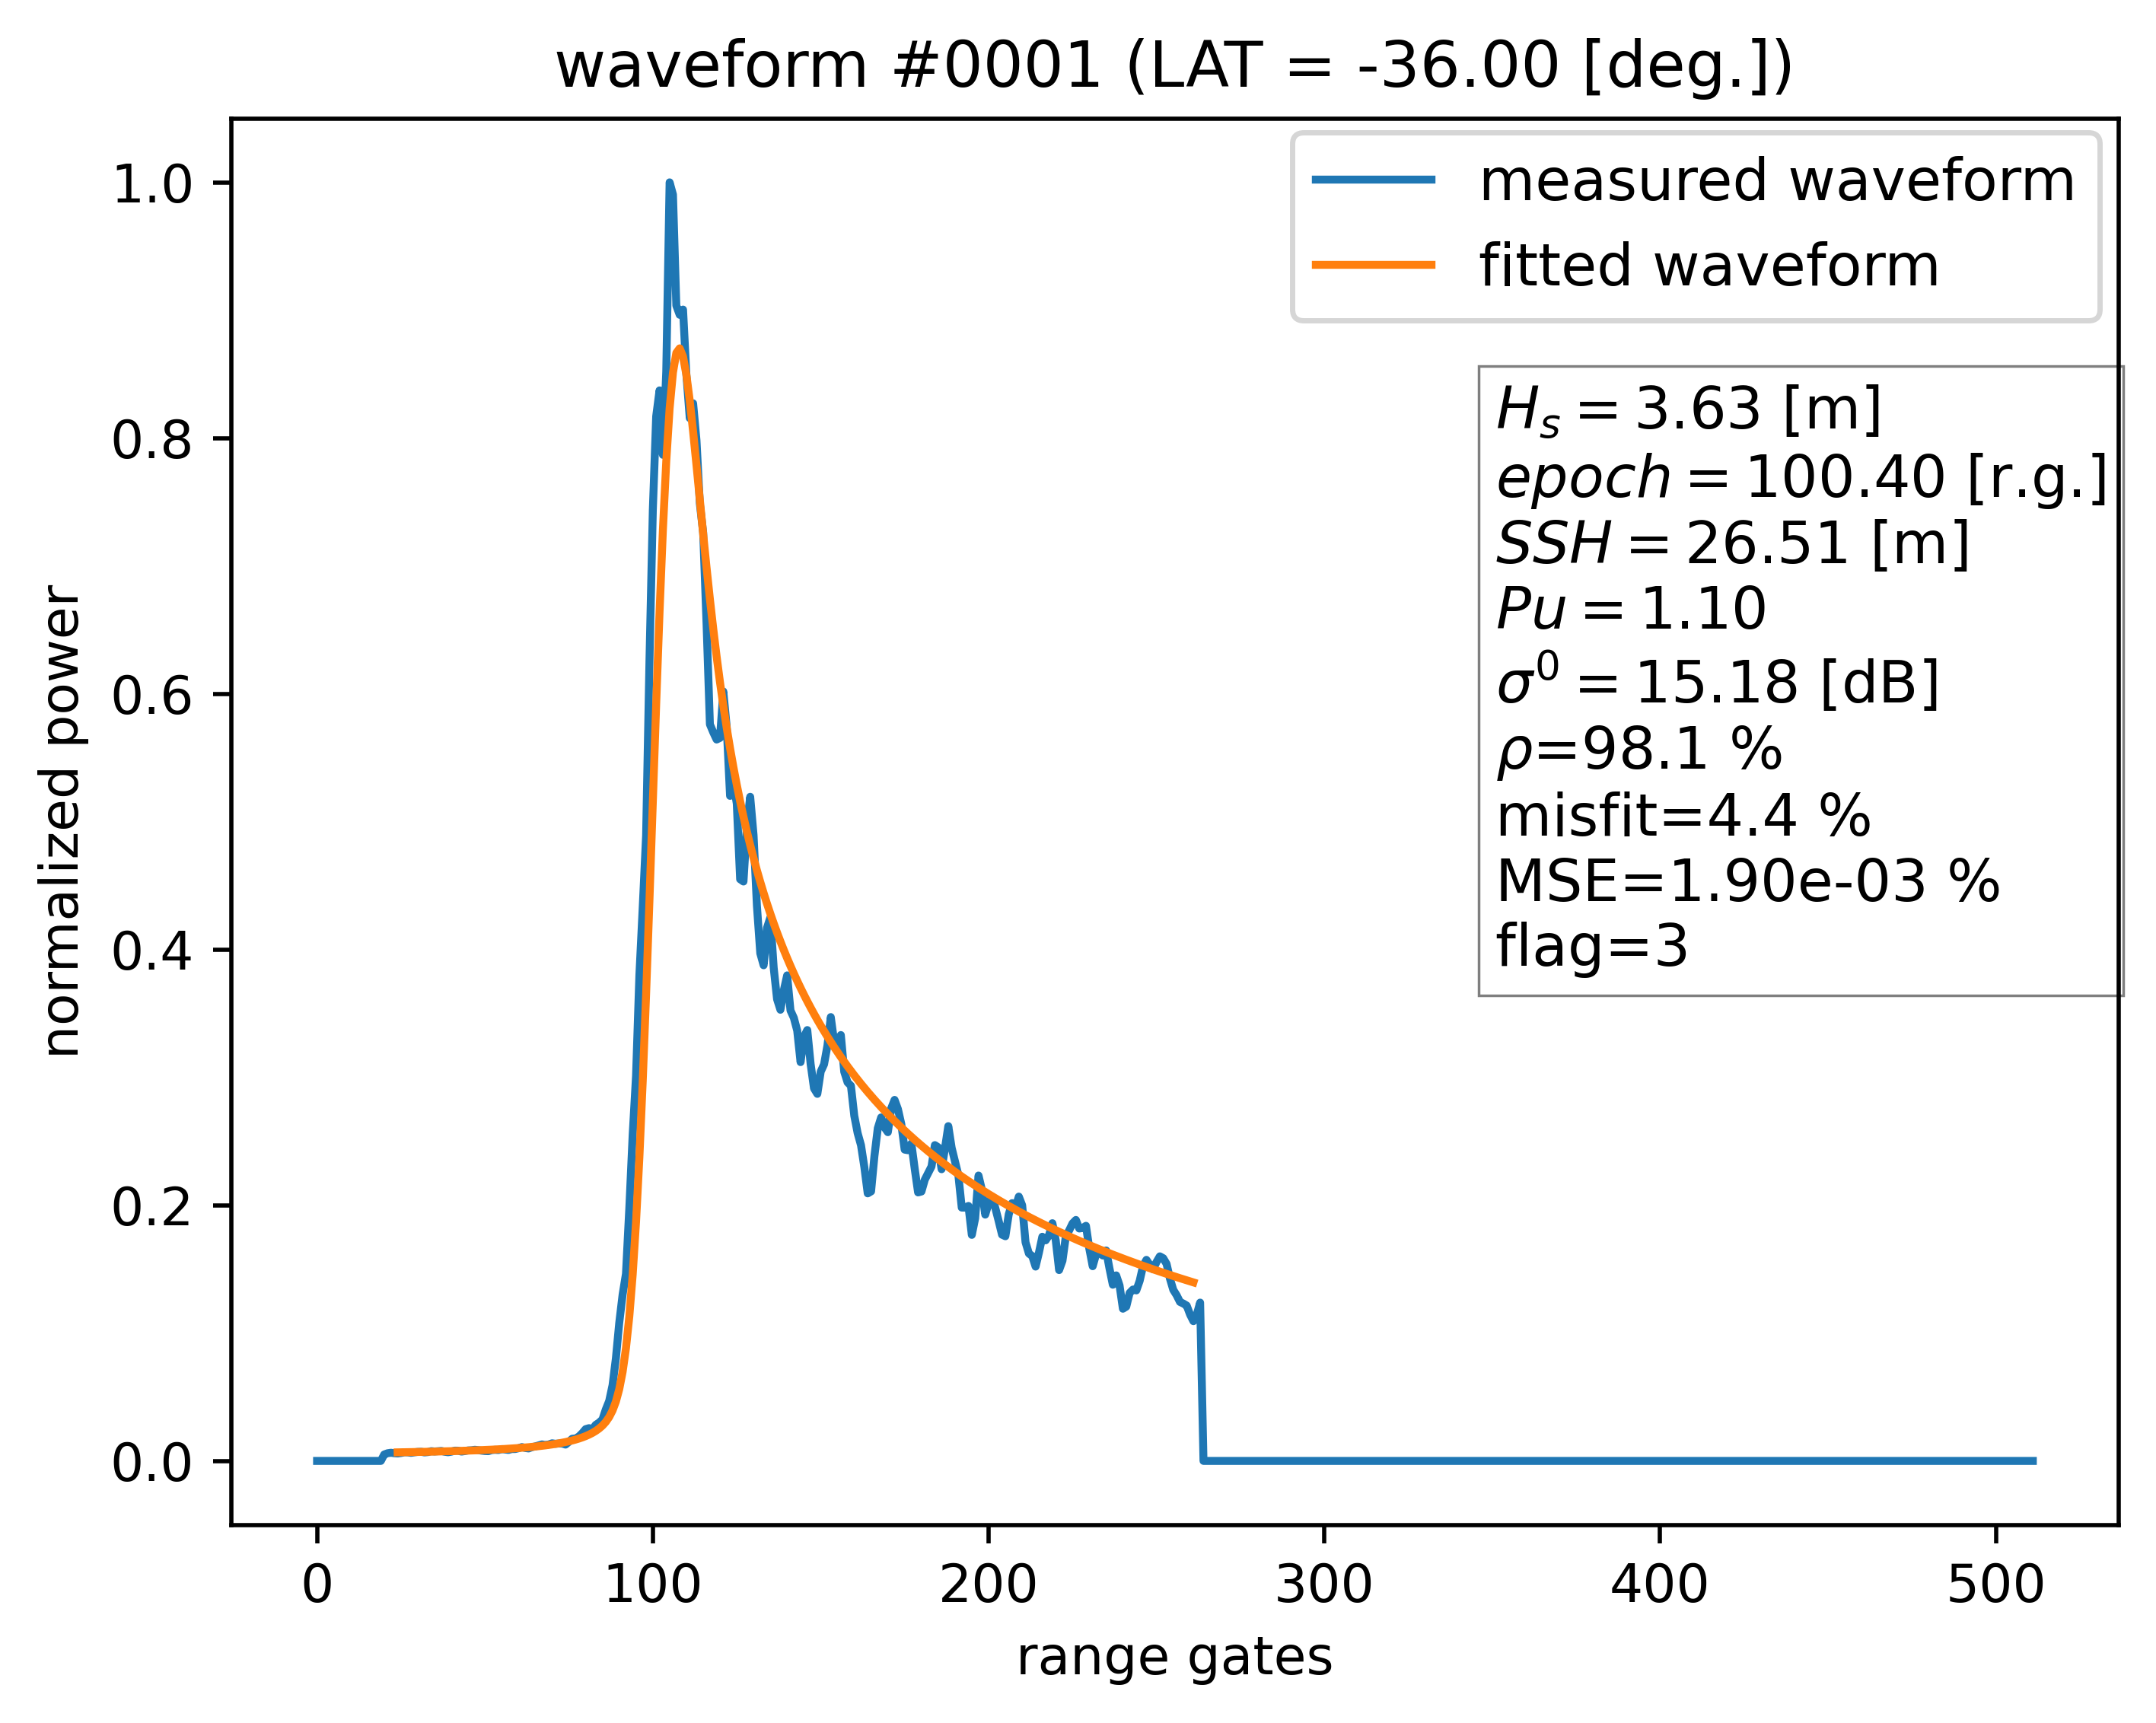
\includegraphics[width=0.7\textwidth]{fig/wfm_1_num_PTRnum_OSAL4}

  az. $4$, $\rho=98.1\%$
  
\end{column}
\begin{column}{0.45\textwidth}\centering

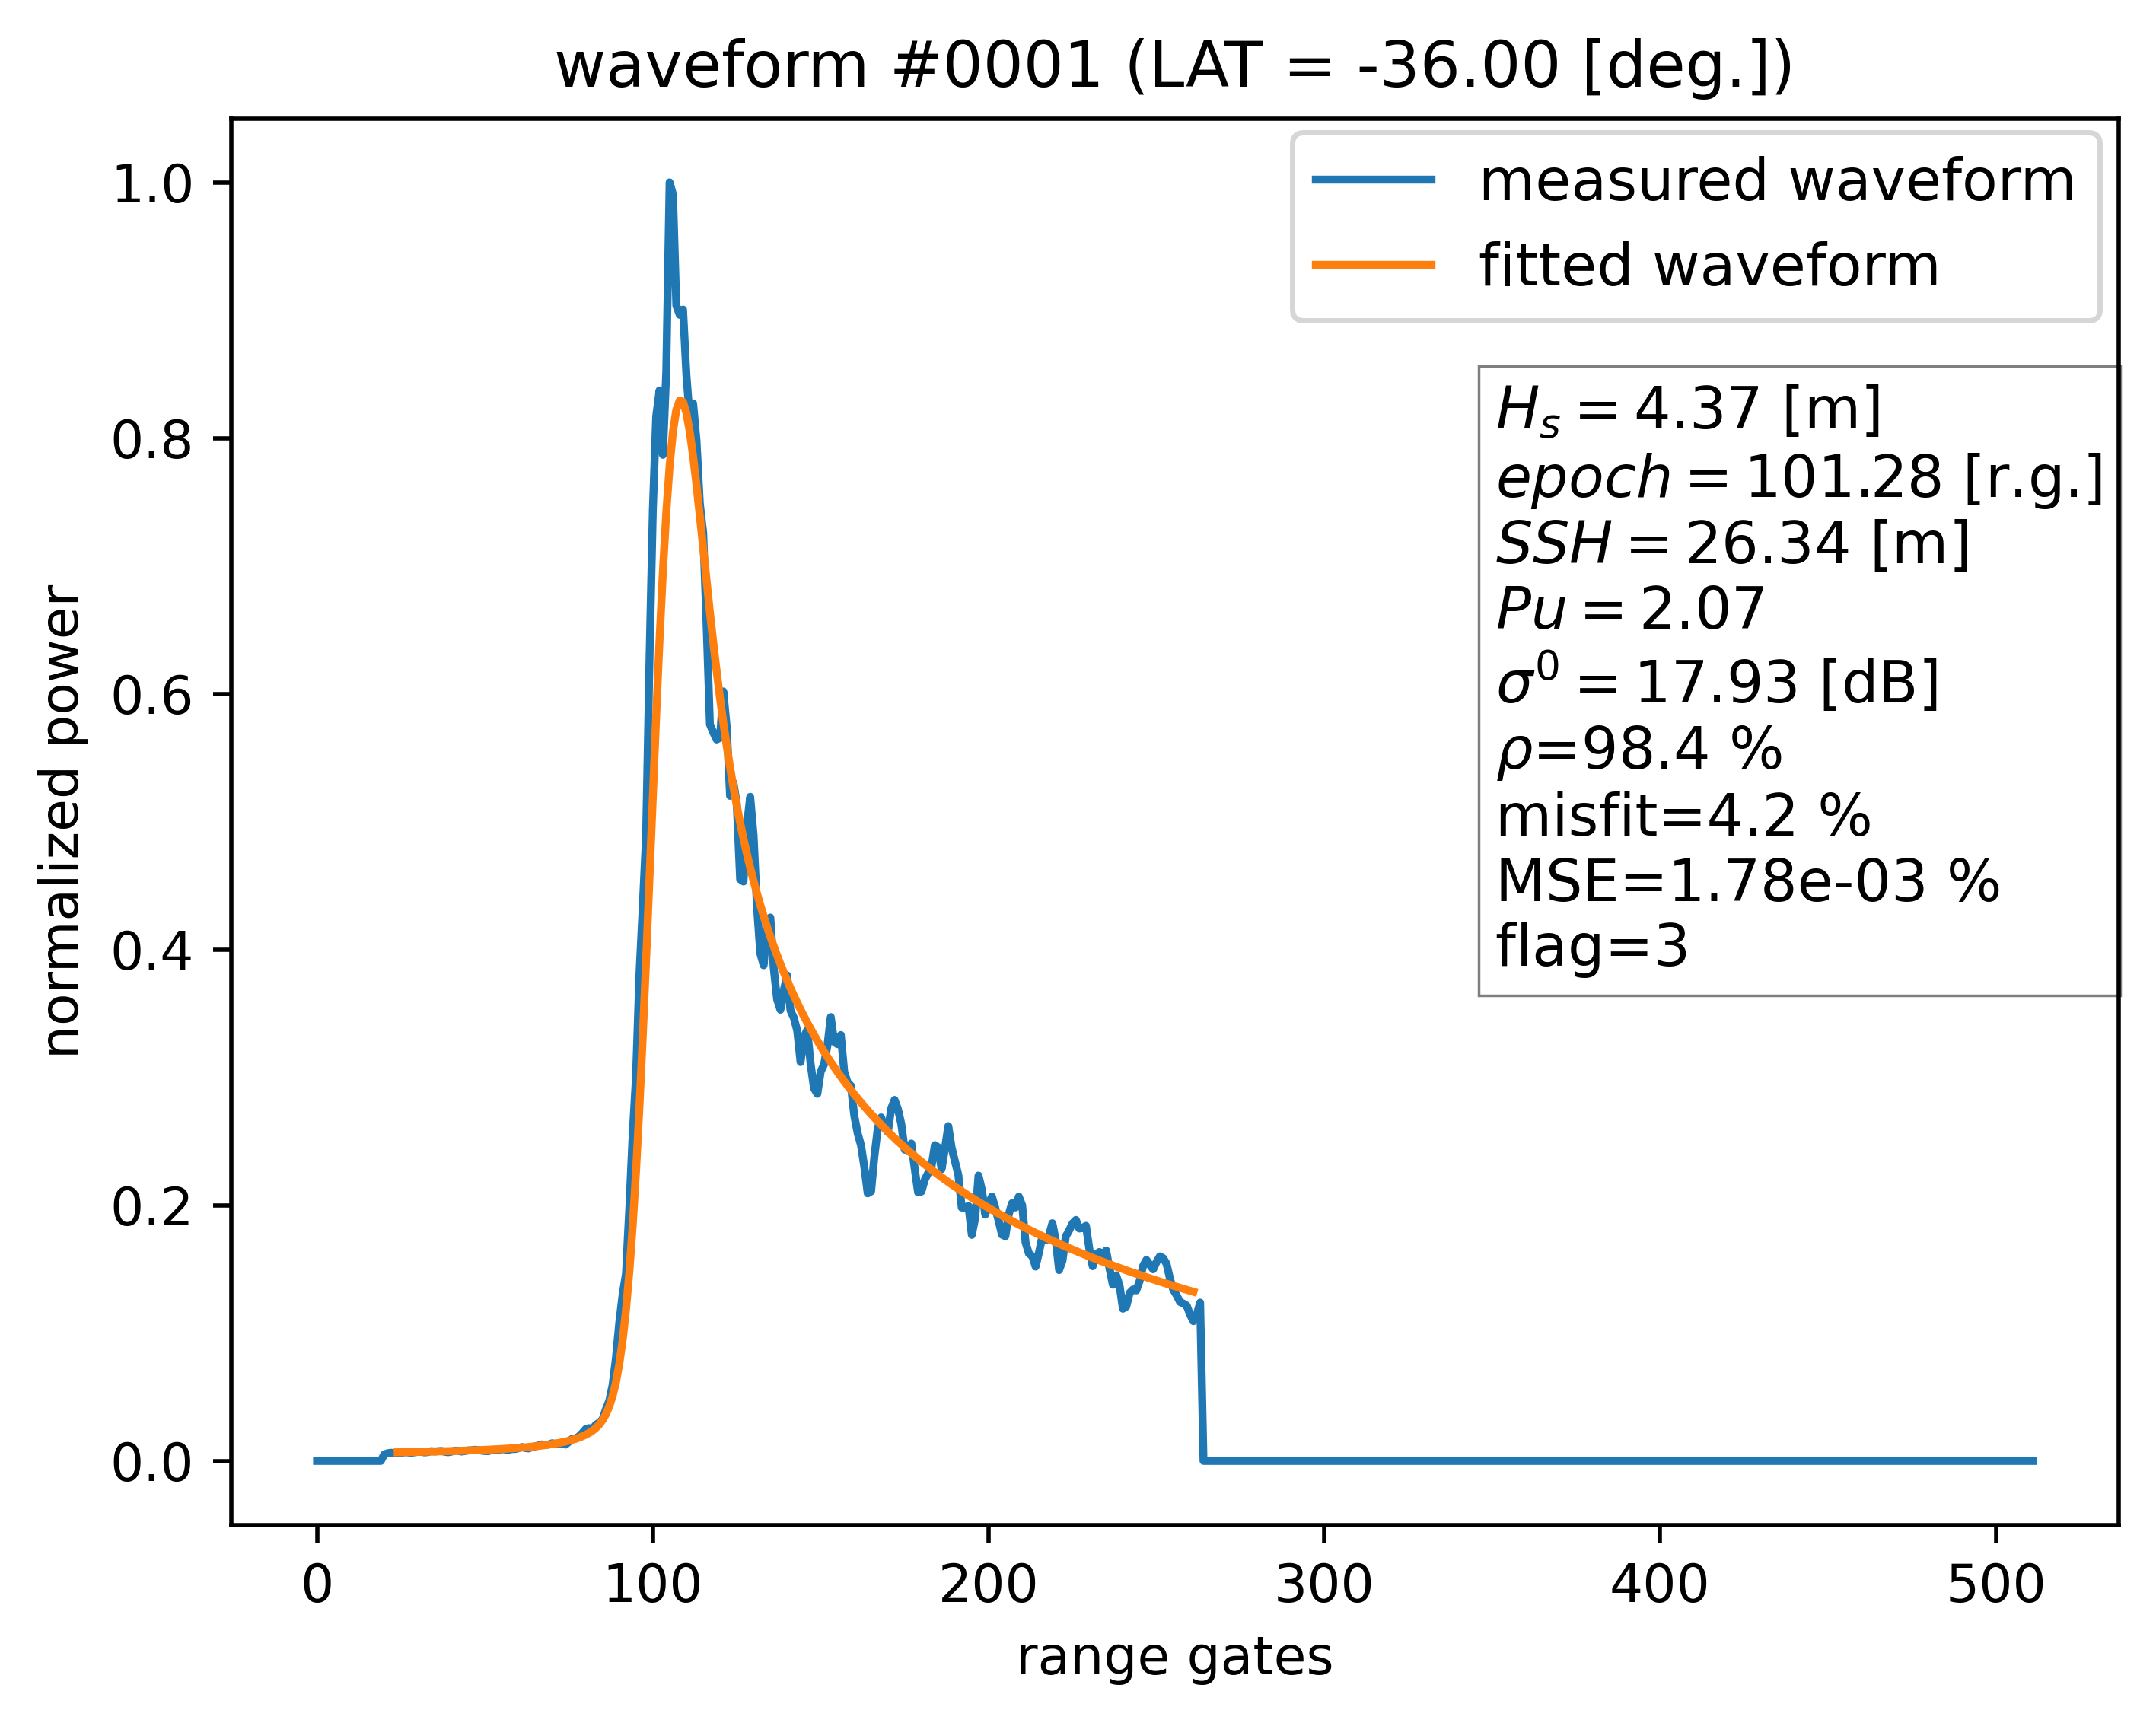
\includegraphics[width=0.7\textwidth]{fig/wfm_1_num_PTRnum_OSAC4} 

ac. $4$,  $\rho=98.4\%$
  
\end{column}
\end{columns}

\medskip
 \begin{columns}
\begin{column}{0.45\textwidth}\centering

  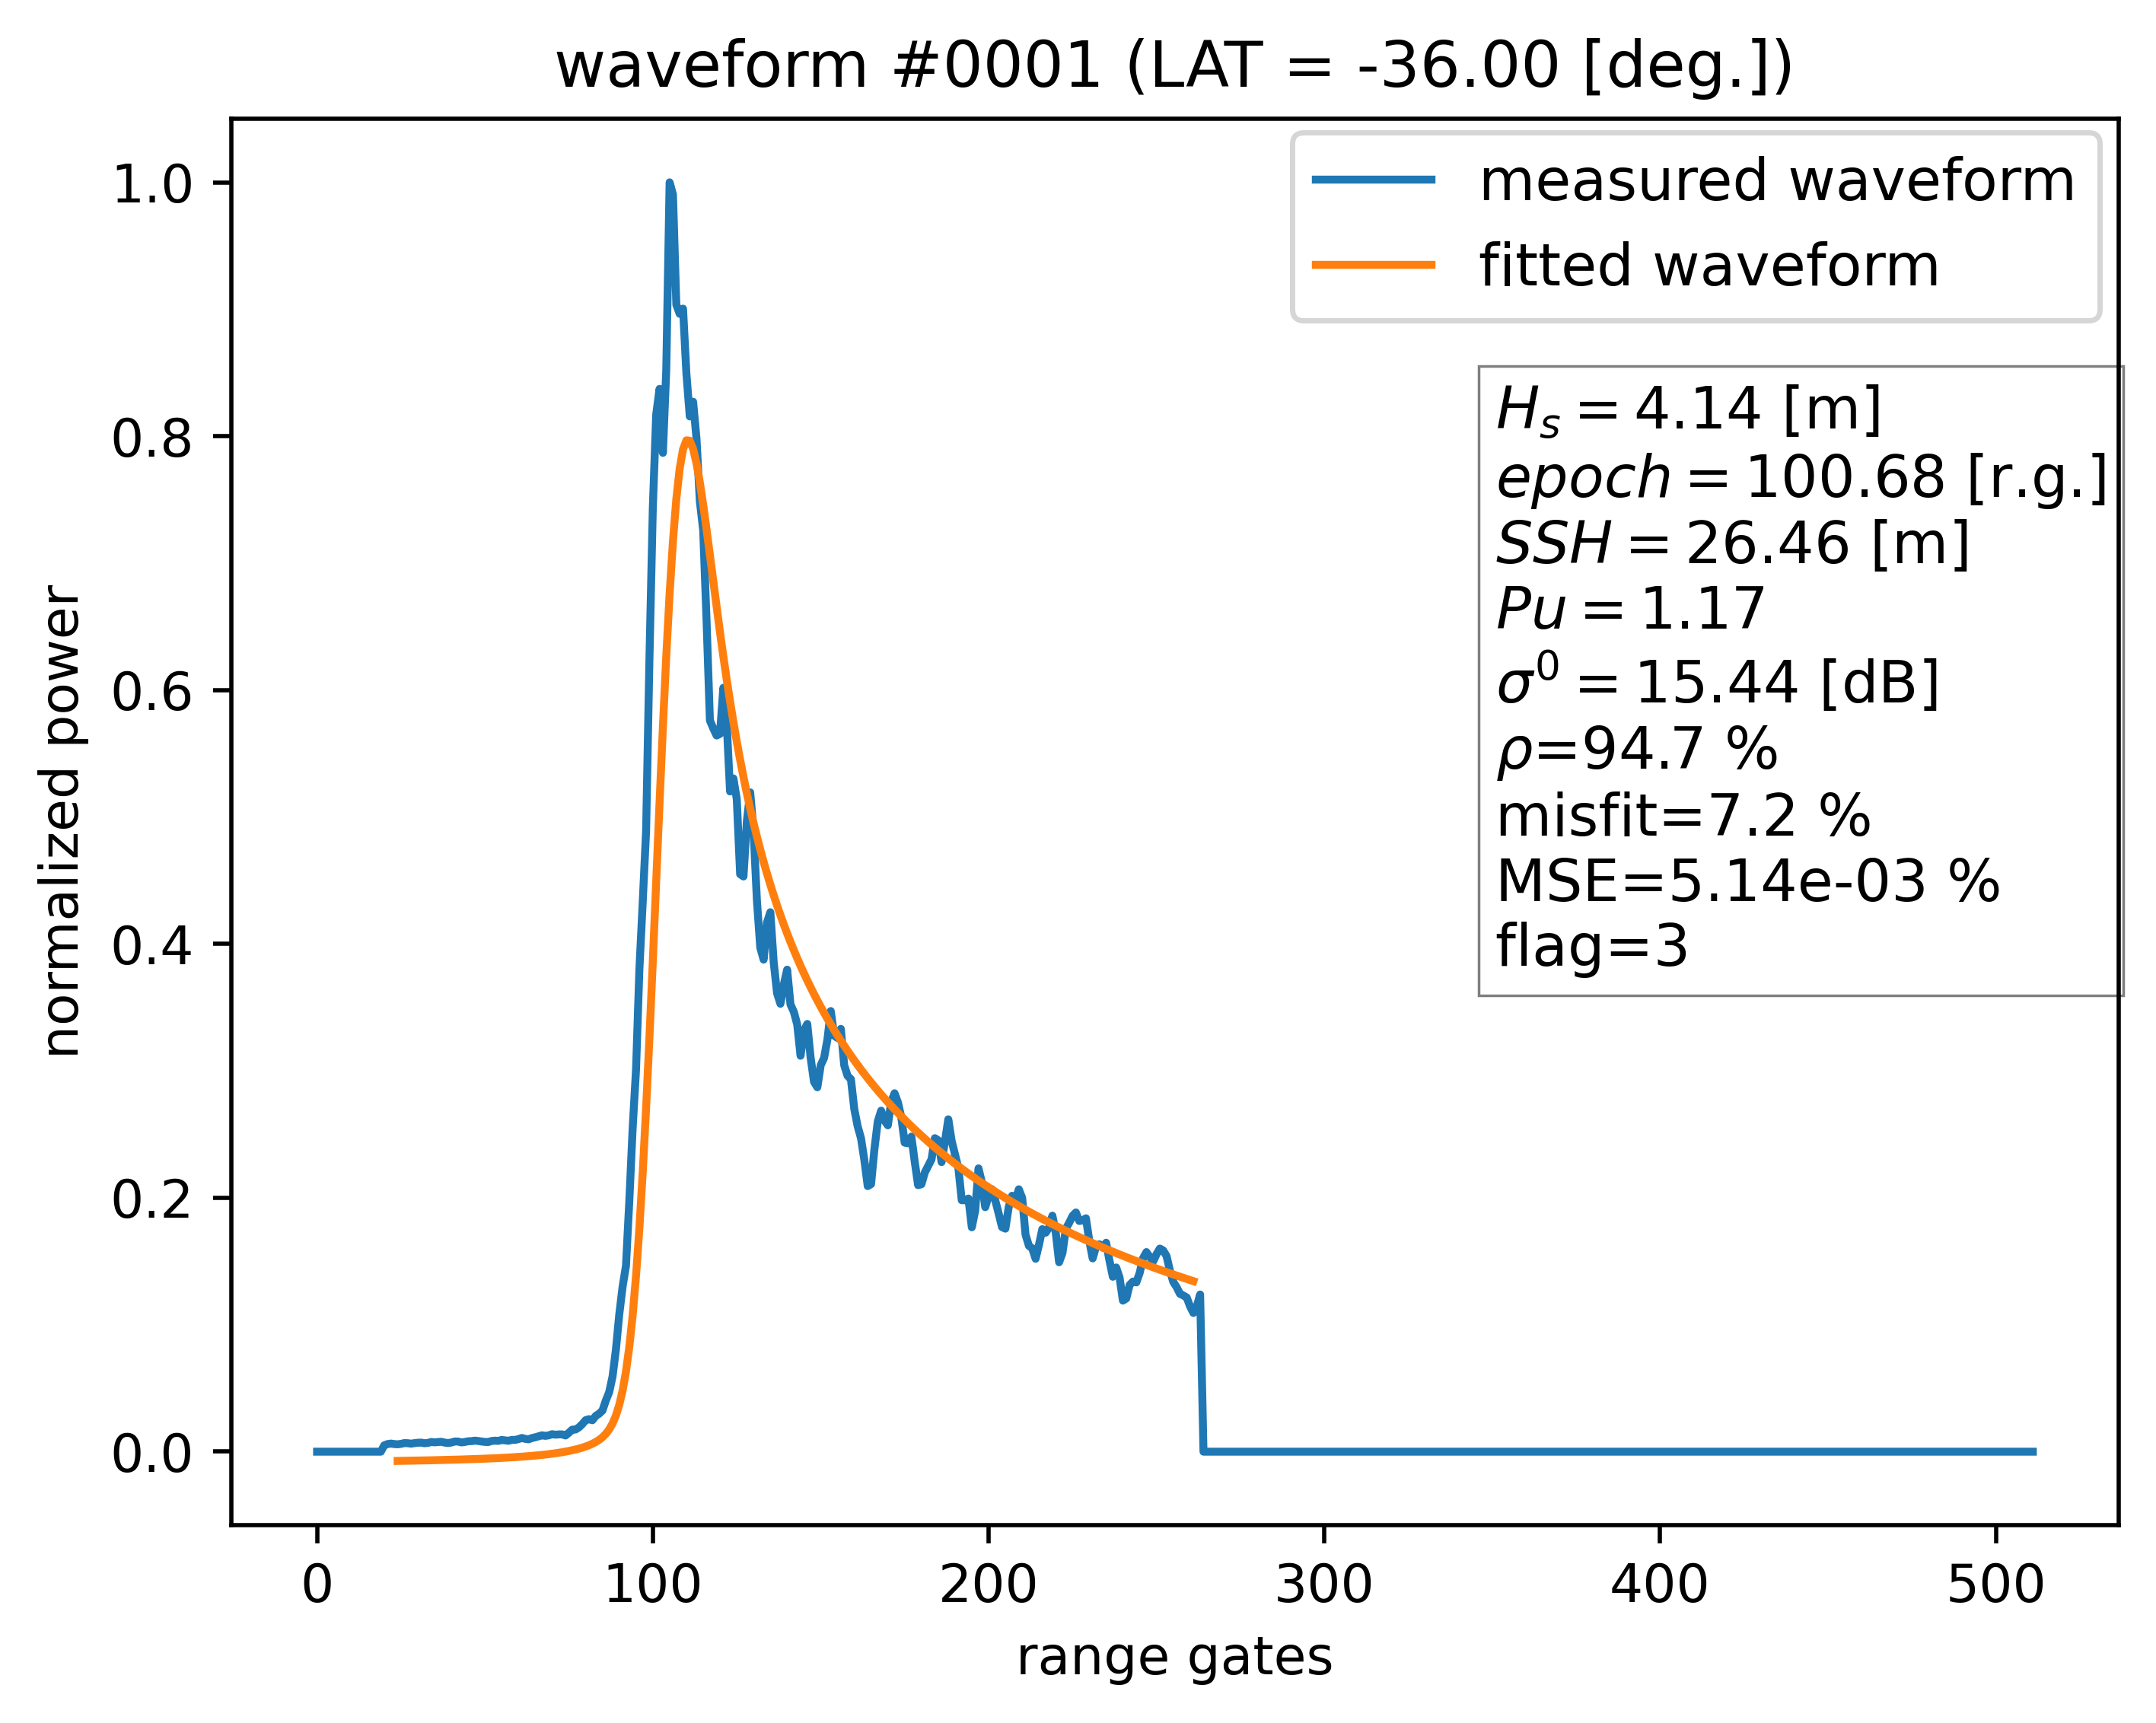
\includegraphics[width=0.7\textwidth]{fig/wfm_1_num_PTRnum_OSAL2}

  az. $2$, $\rho=94.7\%$ 

  
\end{column}
\begin{column}{0.45\textwidth}\centering

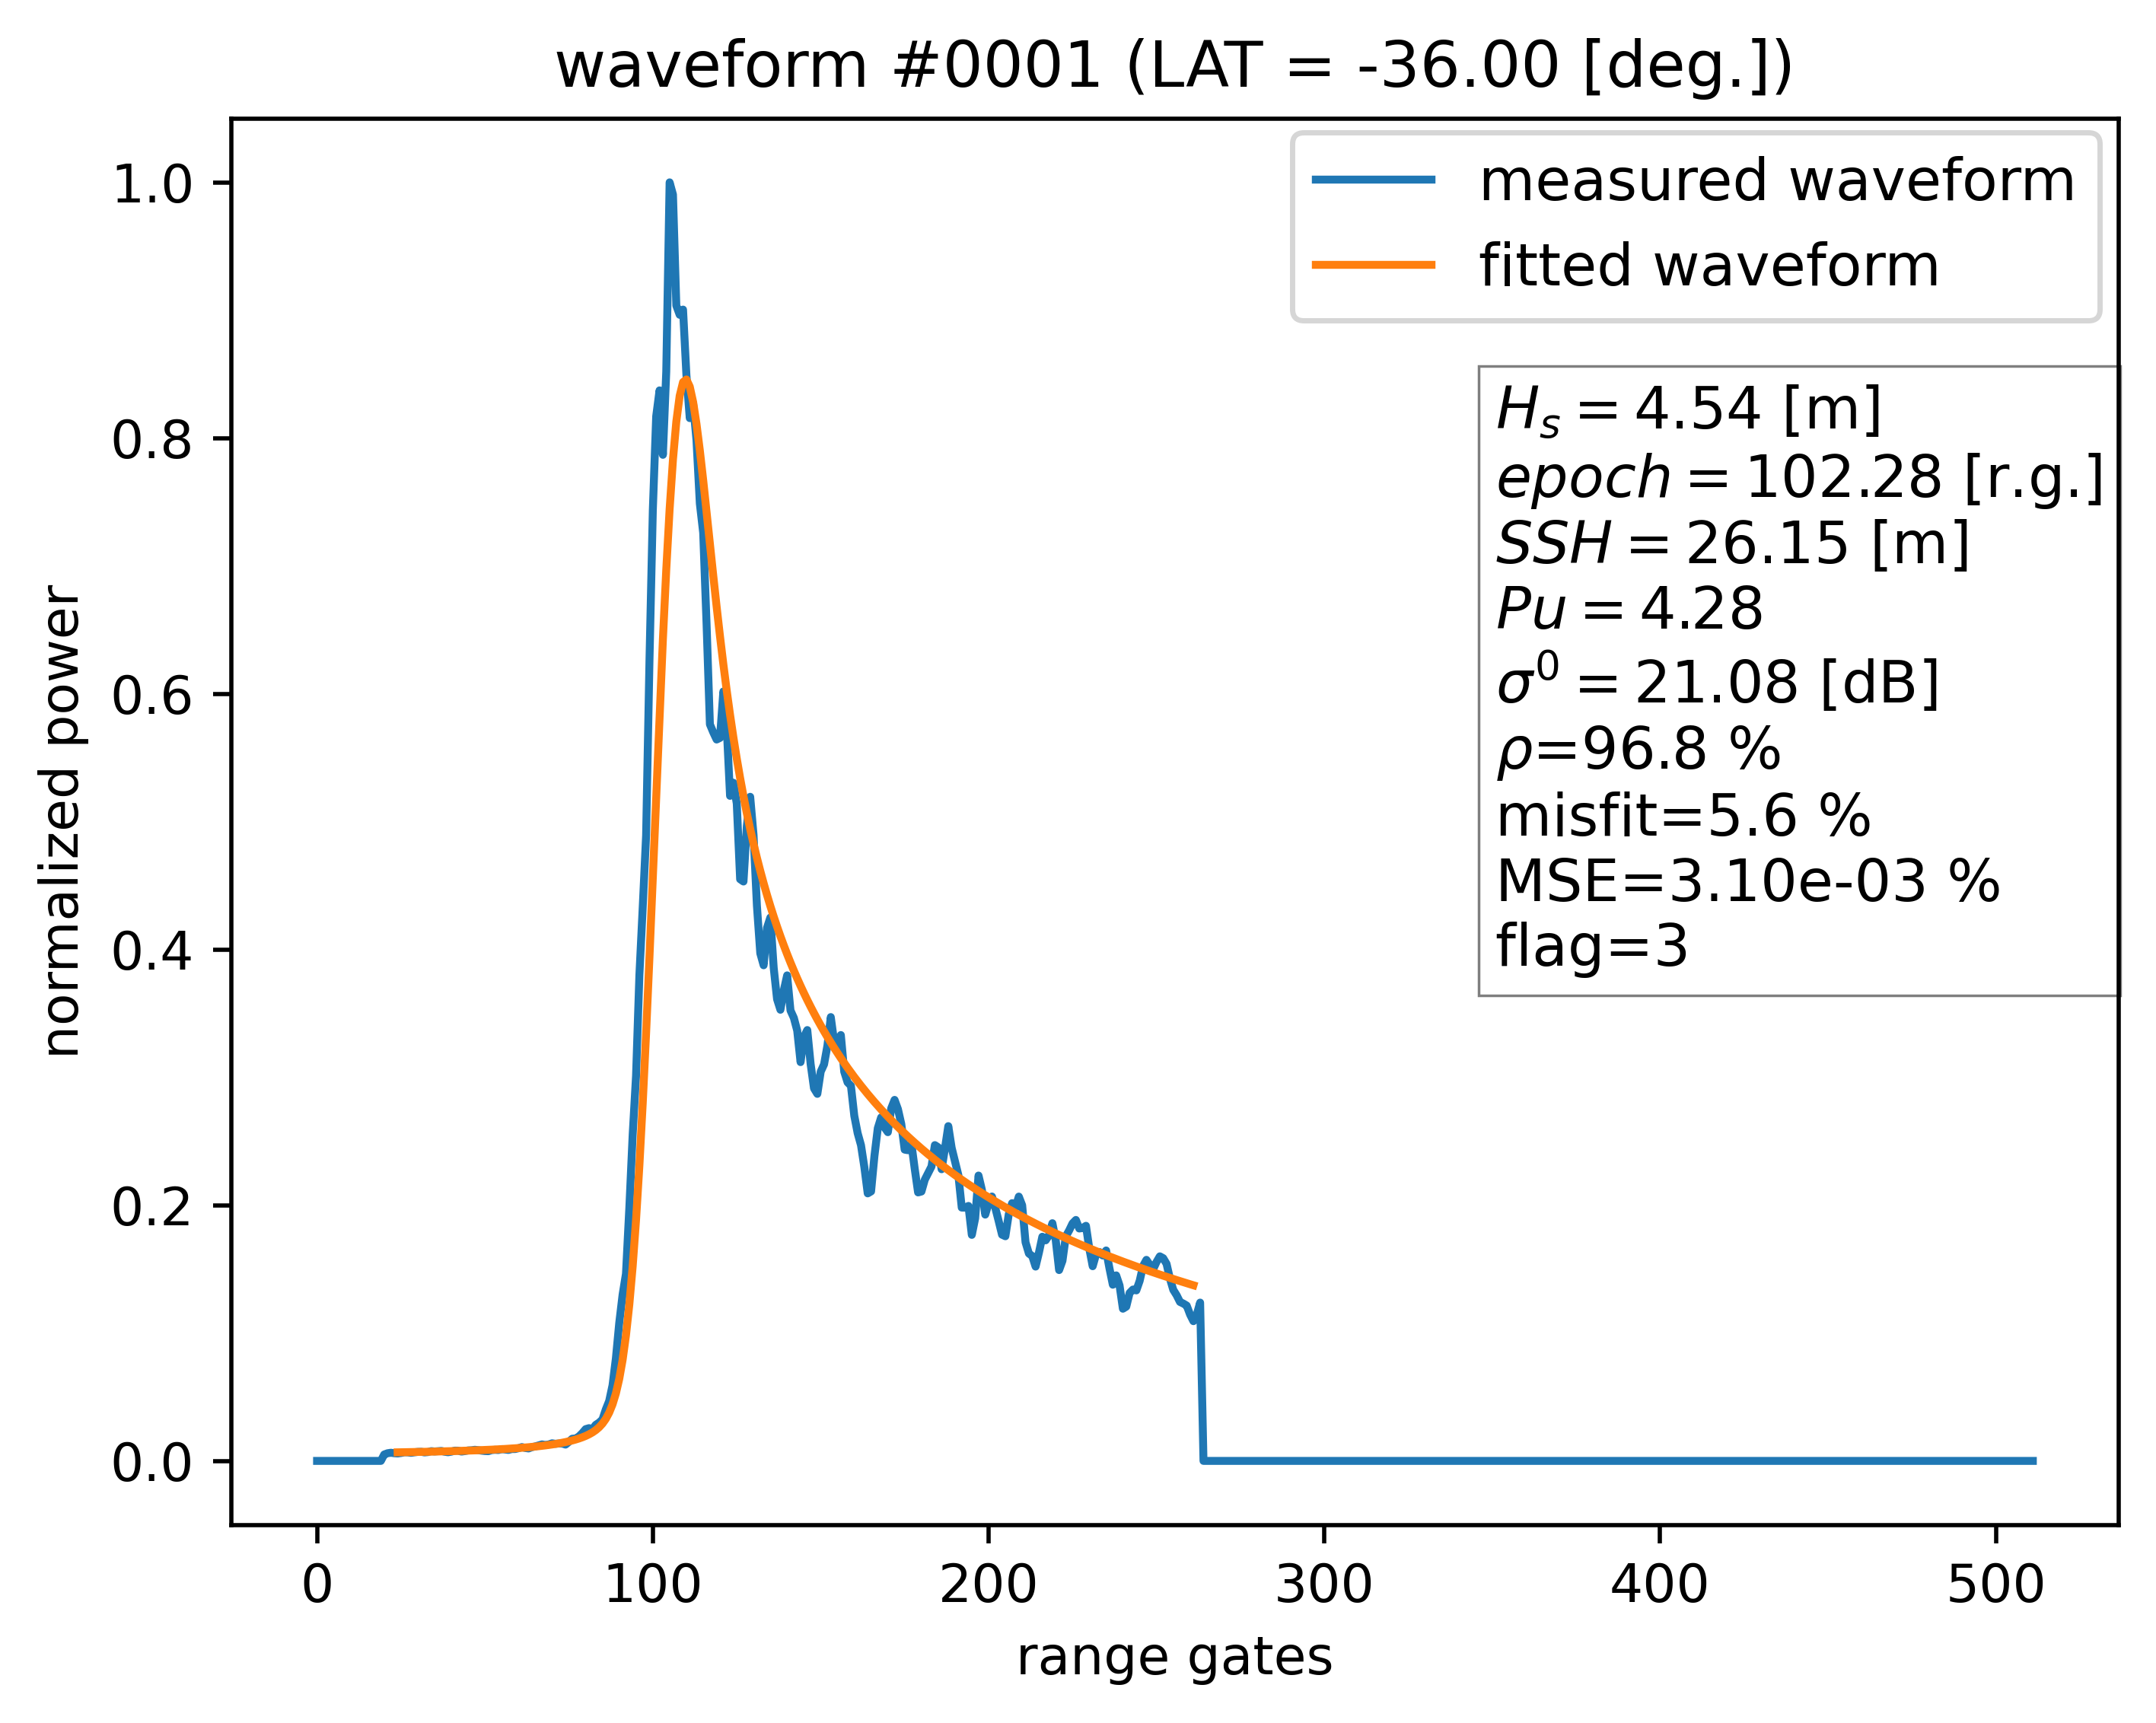
\includegraphics[width=0.7\textwidth]{fig/wfm_1_num_PTRnum_OSAC2} 

ac. $2$, $\rho=96.8\%$ 
  
\end{column}
\end{columns}

\end{frame}




\begin{frame}{Geophysical retrievals series}


 \begin{columns}
\begin{column}{0.5\textwidth}\centering

  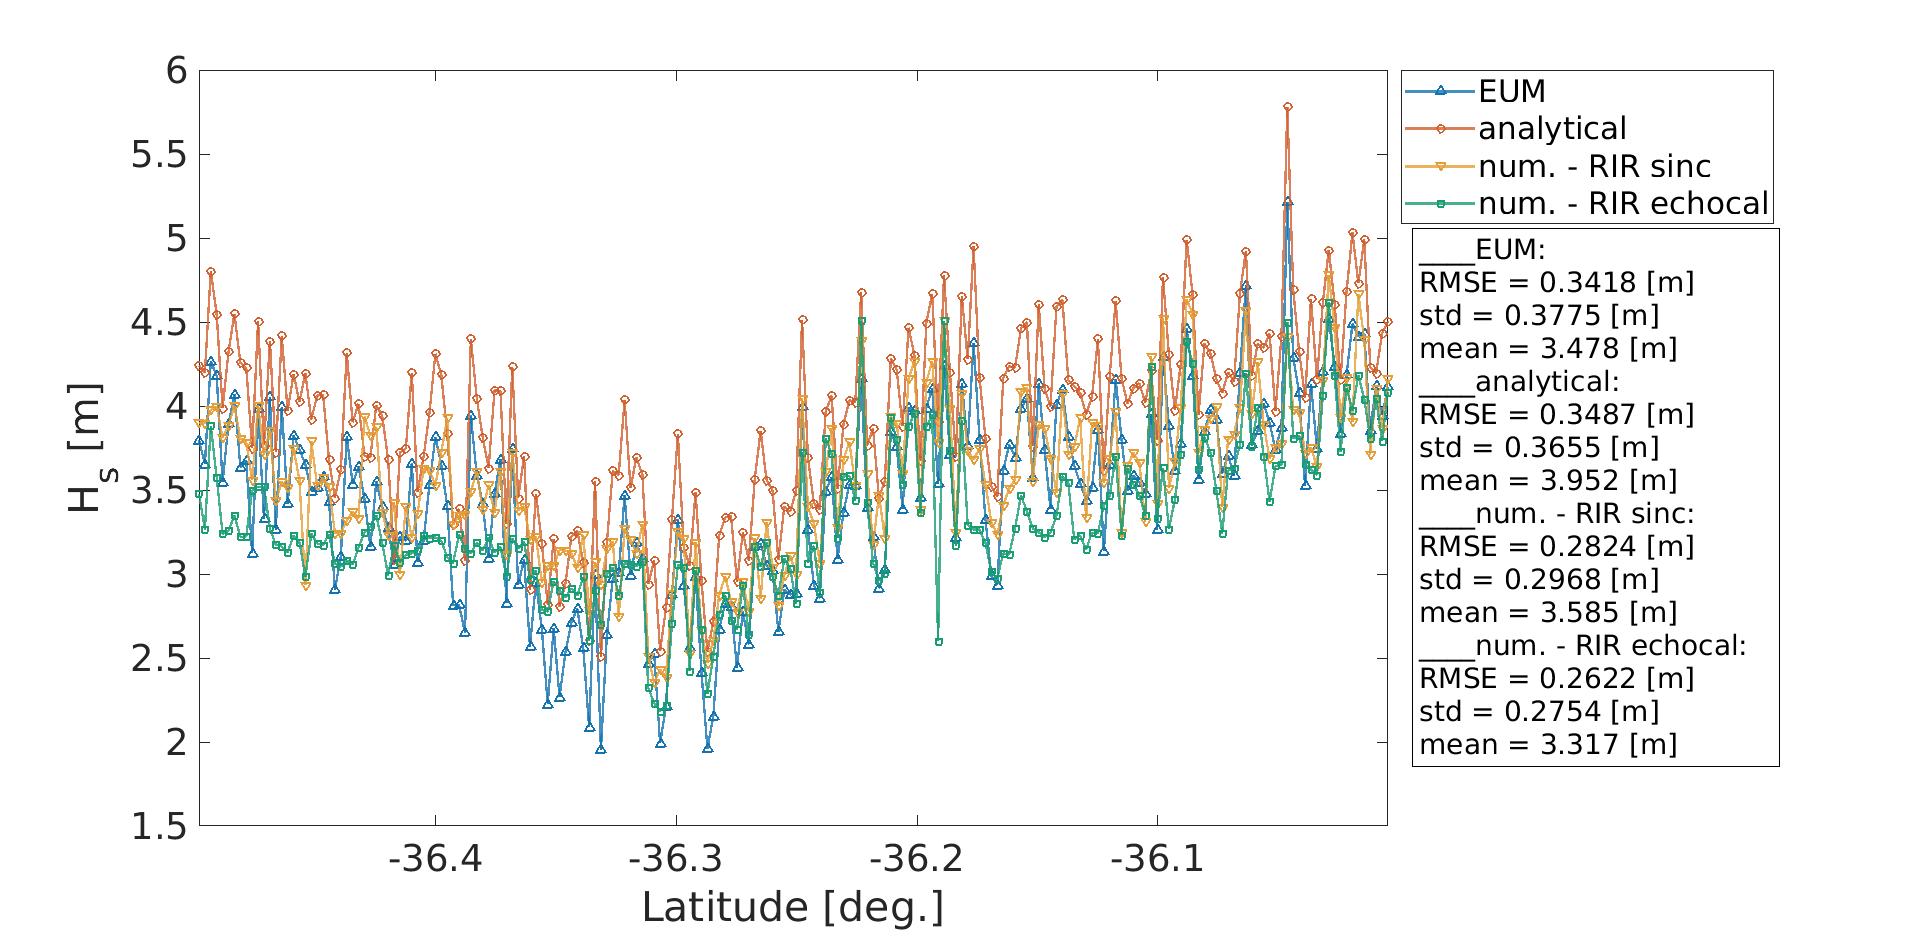
\includegraphics[width=1.1\textwidth]{fig/S6A_P4_2_WAT_HR______20220906T193423_20220906T203036_20220930T170922_3373_067_096_048_EUM__OPE_NT_F07_isd_Hs}

  
\end{column}
\begin{column}{0.5\textwidth}\centering

  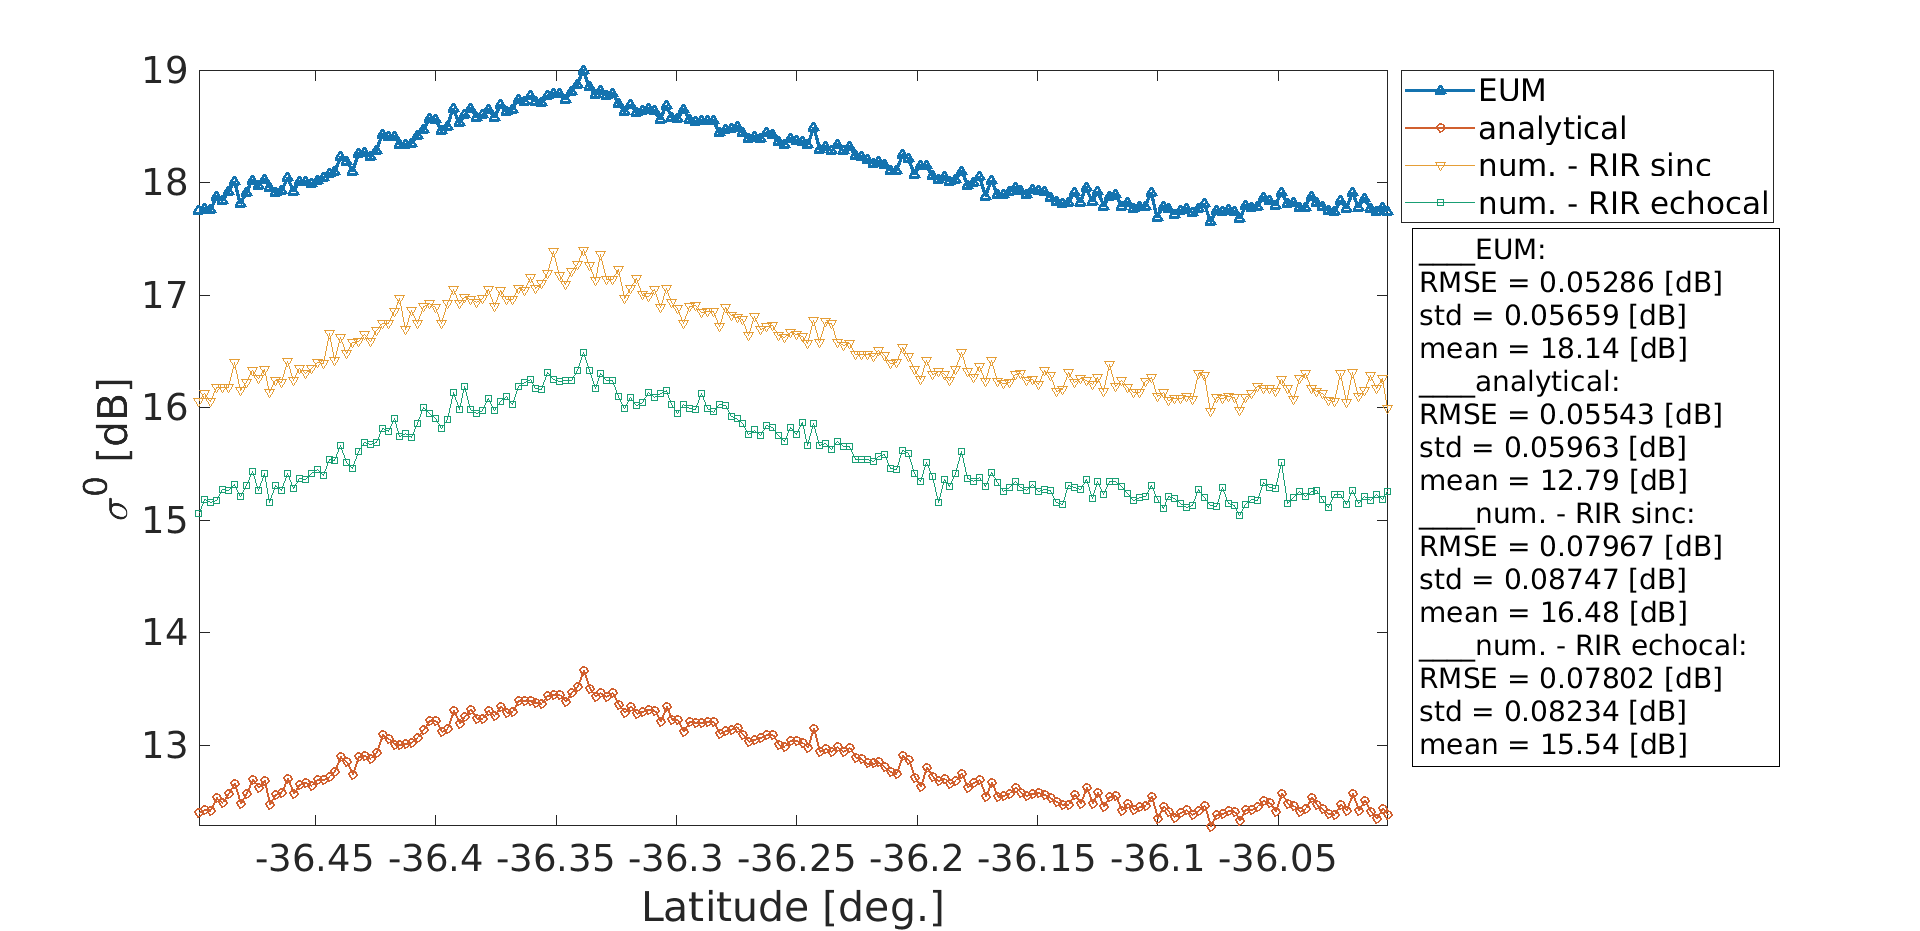
\includegraphics[width=1.1\textwidth]{fig/S6A_P4_2_WAT_HR______20220906T193423_20220906T203036_20220930T170922_3373_067_096_048_EUM__OPE_NT_F07_isd_sigma0}

  
\end{column}
\end{columns}

\medskip
 \begin{columns}
\begin{column}{0.5\textwidth}\centering

  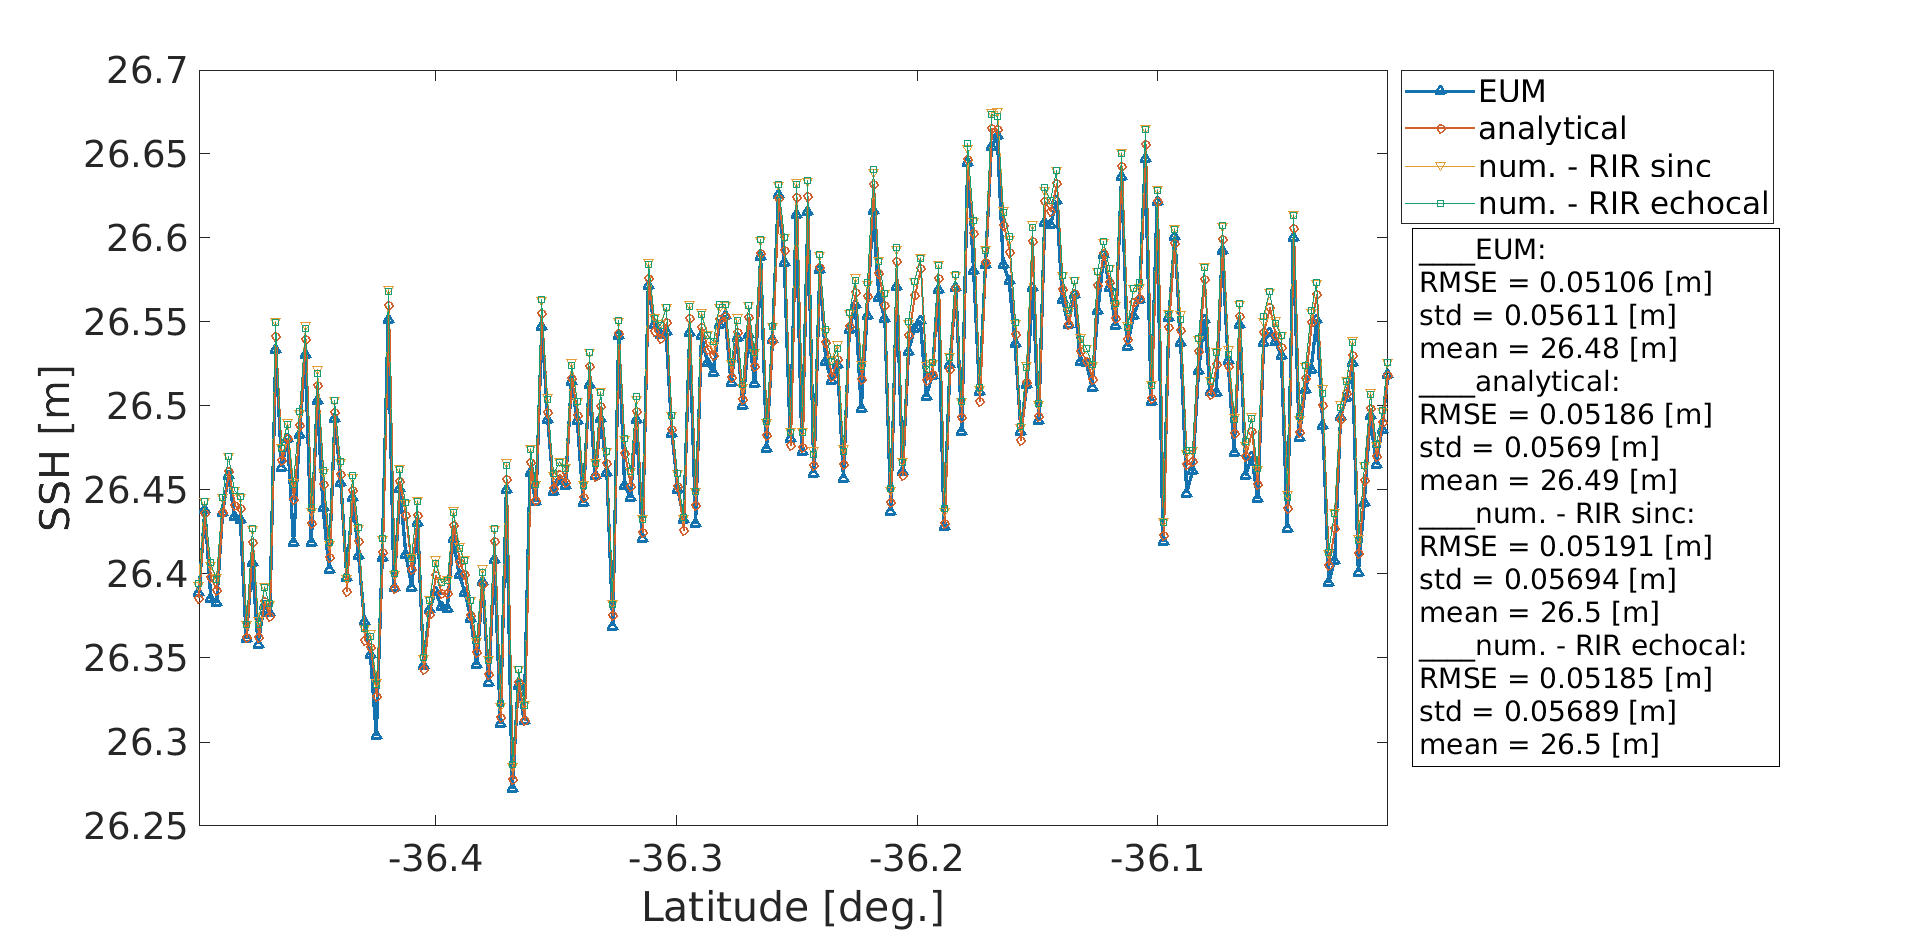
\includegraphics[width=1.1\textwidth]{fig/S6A_P4_2_WAT_HR______20220906T193423_20220906T203036_20220930T170922_3373_067_096_048_EUM__OPE_NT_F07_isd_SSH} 
  
\end{column}
\begin{column}{0.5\textwidth}\centering

\begin{itemize}
 \item Improved precision of $H_s$ with numerical retracker - PTR CAL1.
 \item $H_s$ mean below EUM estimates. Take into account operational LR-HR bias.
 \item Worsen precision of $\sigma^0$ ($\sim 0.03$ dB) with numerical retracker. Existing bias.
 \item SSH results from the numerical retracker are very consistent with results in term of precision. Bias around $\sim 1-2$ cm.
\end{itemize}


  
\end{column}
\end{columns}

\end{frame}



%%%%%%%%%%%%%%%%%%%%%%%%%%%%%%%%%%%%%%%%%%%%%%%%%%%%%%%
\section{Run-time performance}
\begin{frame}

% Fitting On a XXXX machine CPU...

% Architecture:        x86\_64
% 
% factors that affect performance of computer system
% 
% Processor speed: The speed of the processor, measured in GHz
% 
% Memory: The amount and speed of the memory, including RAM
% 
% Time spent executing on the CPU or execution time

The software is run on a Linux OS (Ubuntu 18.04.6 LTS), 64-bit, processor Intel(R) Core(TM) i7-6820HQ CPU @ 2.70GHz $\times$ 8 


\bigskip

The execution times to perform the fitting of one surface are:

\medskip
(default) osversampling (os) along track (al) $10$ and os across track (ac) $8$ $= 51$ sec

\begin{itemize}
 \item os al $4$ and os ac $8$ $= 32$ sec

 \item os al $2$ and os ac $8$ $= 27$ sec

 \item os al $10$ and os ac $4$ $= 41$ sec

 \item os al $10$ and os ac $2$ $= 13$ sec

 \item os al $1$ and os ac $1$ $= 2$ sec

\end{itemize}


\end{frame}





%%%%%%%%%%%%%%%%%%%%%%%%%%%%%%%%%%%%%%%%%%%%%%%%%%%%%%%%%%%%%%%%%%%%%
\section{Conclusions and next steps}
 \begin{frame}

 \begin{block}{}
\textbf{Conclusions}
\end{block}
 
\begin{itemize}
\item Results show no large differences between numerical retracker model with modelled and measured RIR, for this particular set of points.
\item Results show improvement of $H_s$ precision with the numerical retracker, better for measured PTR. Also, a decrease in the mean with respect to L2 operational product.

\item $\sigma^0$ retrieval slightly worsen the precision by $\sim 0.3$ dB

\item Range estimates are consistent with analytical retrackers outputs, although a slight bias is detected.

 \item High sensitivity of the retracker output to oversampling.

 \item Sensitivity to initial parameters choice is also detected.
 
  \item Theses conclusion shall be taken with caution, since the dataset analysed here is small.


 \item The oversampling is the main factor affecting execution times, thought the numerical convolution operation.
 
\end{itemize}

\vspace{-0.3cm  }
 \begin{block}{}
\textbf{Next steps}
\end{block}

\begin{itemize}

\item Full assessment over one cycle of data.

\item Investigate possible strategies to reduce execution times.

\item Investigate biases.

\end{itemize}

\end{frame}





% %%%%%%%%%%%%%%%%%%%%%%%%%%%%%%%%%%%%%%%%%%%%%%%%%%%%%%%%%%%%%%%%%%%%%%%%%%%%%
{
\usebackgroundtemplate{
\includegraphics[width=\paperwidth]{fig/backcover_isardsat}}
\begin{frame}[plain]
 
 \begin{center}
 \Large End of presentation
  \end{center}
  
\end{frame}
}



\section*{}
\begin{frame}


\textbf{References}

\bigskip

\tiny
 %%%%%%%%%%%%%%%%%%%%%%%%%%%%%%%%%%%%%%%%%%%%%%
\bibliography{library.bib}
 
\end{frame}


\end{document}
